\documentclass[sigconf,nonacm]{acmart}

\usepackage{tikz}
\usepackage[nameinlink,capitalise,noabbrev]{cleveref}
\usepackage{hyperref}
\usepackage{microtype}
\usepackage{enumerate}
\usepackage{enumitem}
\usepackage{todonotes}
\usepackage{xfrac}
\usepackage{pifont}
\usepackage{adjustbox}

\newcommand{\cmark}{\ding{51}}%
\newcommand{\xmark}{\ding{55}}%

\newcounter{cccnt}
\newcounter{bdscnt}
\newcounter{rgcnt}
\newcounter{bccnt}

\newcommand{\cc}[1]{\refstepcounter{cccnt}
	\textcolor{purple}{\textbf{CC: [\thecccnt]:} #1}}
\newcommand{\bds}[1]{\refstepcounter{bdscnt}
	\textcolor{pink}{\textbf{BDS: [\thebdscnt]:} #1}}
\newcommand{\rg}[1]{\refstepcounter{rgcnt}
	\textcolor{red}{\textbf{RG: [\thetfcnt]:} #1}}
\newcommand{\bc}[1]{\refstepcounter{bccnt}
	\textcolor{blue}{\textbf{BC [\thebccnt]:} #1}}


\newcommand*\circledw[1]{\tikz[baseline=(char.base)]{
		\node[shape=circle,draw,inner sep=.75pt, line width=.7pt] (char) {\scriptsize #1};}}
\newcommand*\dcircledw[1]{\tikz[baseline=(char.base)]{
		\node[shape=circle,draw,dashed,dash pattern = on 1.5pt off .75pt, inner sep=.75pt, line width=.7pt] (char) {\scriptsize #1};}}

\newcommand*\recdw[1]{\tikz[baseline=(char.base)]{
		\node[shape=rectangle,draw,inner sep=0.18em, line width=.7pt] (char) {\scriptsize #1};}}
\newcommand*\drecdw[1]{\tikz[baseline=(char.base)]{
		\node[shape=rectangle,draw,dashed,dash pattern = on 1.5pt off .75pt, inner sep=0.18em, line width=.7pt] (char) {\scriptsize #1};}}


\widowpenalty=10000
\clubpenalty=10000
\brokenpenalty=10000

\renewenvironment{quote}{%
  \list{}{%
    \leftmargin0.5cm   % this is the adjusting screw
    \rightmargin0.05cm
  }
  \item\relax
}
{\endlist}

\hyphenation{Rev-Eng}

%%
%% \BibTeX command to typeset BibTeX logo in the docs
\AtBeginDocument{%
  \providecommand\BibTeX{{%
    Bib\TeX}}}

%% Rights management information.  This information is sent to you
%% when you complete the rights form.  These commands have SAMPLE
%% values in them; it is your responsibility as an author to replace
%% the commands and values with those provided to you when you
%% complete the rights form.
%% These commands are for a PROCEEDINGS abstract or paper.
%% TODO from rights form?


%\copyrightyear{2024}
%\acmYear{2024}
%\setcopyright{acmlicensed}\acmConference[shorthand]{full booktitle}{date}{location}
%\acmBooktitle{full booktitle (shorthand), date, location}
%\acmPrice{TODO}
%\acmDOI{TODO}
%\acmISBN{TODO}

%%
%% Submission ID.
%% Use this when submitting an article to a sponsored event. You'll
%% receive a unique submission ID from the organizers
%% of the event, and this ID should be used as the parameter to this command.
%%\acmSubmissionID{123-A56-BU3}

%%
%% For managing citations, it is recommended to use bibliography
%% files in BibTeX format.
%%
%% You can then either use BibTeX with the ACM-Reference-Format style,
%% or BibLaTeX with the acmnumeric or acmauthoryear sytles, that include
%% support for advanced citation of software artefact from the
%% biblatex-software package, also separately available on CTAN.
%%
%% Look at the sample-*-biblatex.tex files for templates showcasing
%% the biblatex styles.
%%

%%
%% The majority of ACM publications use numbered citations and
%% references.  The command \citestyle{authoryear} switches to the
%% "author year" style.
%%
%% If you are preparing content for an event
%% sponsored by ACM SIGGRAPH, you must use the "author year" style of
%% citations and references.
%% Uncommenting
%% the next command will enable that style.
%%\citestyle{acmauthoryear}


%%
%% end of the preamble, start of the body of the document source.
\begin{document}

%%
%% The "title" command has an optional parameter,
%% allowing the author to define a "short title" to be used in page headers.

\title{A New Framework of Software Obfuscation Evaluation Criteria}

%\author{Anonymous}
\author{Bjorn De Sutter}
\email{bjorn.desutter@ugent.be}
\orcid{0000-0003-0317-2089}
\affiliation{
\institution{Ghent University}
\city{Ghent}
\country{Belgium}
}

%\author{Anyone willing to contribute}

%%
%% By default, the full list of authors will be used in the page
%% headers. Often, this list is too long, and will overlap
%% other information printed in the page headers. This command allows
%% the author to define a more concise list
%% of authors' names for this purpose.
% \renewcommand{\shortauthors}{De Ghein et al.}

%%
%% The abstract is a short summary of the work to be presented in the
%% article.
\begin{abstract}
In the domain of practical software protection against man-at-the-end attacks such as software reverse engineering and tampering, much of the scientific literature is plagued by the use of subpar methods to evaluate the protections' strength and even by the absence of such evaluations. Several criteria have been proposed in the past to assess the strength of protections, such as potency, resilience, stealth, and cost. We analyze their evolving definitions and uses. We formulate a number of critiques, from which we conclude that the existing definitions are unsatisfactory and need to be revised. We present a new framework of software protection evaluation criteria: relevance, effectiveness (or efficacy), robustness, concealment, stubbornness, sensitivity, predictability, and cost.
\end{abstract}

%%
%% The code below is generated by the tool at http://dl.acm.org/ccs.cfm.
%% Please copy and paste the code instead of the example below.
%%
\begin{CCSXML}
<ccs2012>
<concept>
<concept_id>10002978.10003022.10003465</concept_id>
<concept_desc>Security and privacy~Software reverse engineering</concept_desc>
<concept_significance>500</concept_significance>
</concept>
</ccs2012>
\end{CCSXML}

\ccsdesc[500]{Security and privacy~Software reverse engineering}

%%
%% Keywords. The author(s) should pick words that accurately describe
%% the work being presented. Separate the keywords with commas.
\keywords{Potency, resilience, stealth, obfuscation, attacks, program analysis}
%% A "teaser" image appears between the author and affiliation
%% information and the body of the document, and typically spans the
%% page.
% \begin{teaserfigure}
%   \includegraphics[width=\textwidth]{sampleteaser}
%   \caption{Seattle Mariners at Spring Training, 2010.}
%   \Description{Enjoying the baseball game from the third-base
%   seats. Ichiro Suzuki preparing to bat.}
%   \label{fig:teaser}
% \end{teaserfigure}

%%
%% This command processes the author and affiliation and title
%% information and builds the first part of the formatted document.
\maketitle


% Alphabetical:
% \belfius
% \payconiq
% \argenta
% \axa
% \kbc
% \ING
% \beobank
% \keytrade
% \bpost
% \crelan
% newcolumn
% \bunq
% \knab
% \vdk
% \fortis
% \abnamro
% \delen
% \breda
% \ASN
% \rabobank
% \SNS

\newcommand{\defeq}{\overset{\mathrm{def}}{=}}

\documentclass[../main.tex]{subfiles}
\graphicspath{{../images/}}
\makeatletter
\def\input@path{{../images/}}
\makeatother
\begin{document}
\section{Introduction}
\begin{figure}
\centering
\begin{tikzpicture}
\node[inner sep=0pt] (ws) at (0, 0) {
\includegraphics[height=.4\textwidth, trim={10cm 0 10cm 0},clip]{world_space.png}};
\node[inner sep=0pt] (cs) at (6,0) {\includegraphics[height=.4\textwidth, trim={10cm 1cm 10cm 4cm},clip]{conf_space.png}};
\end{tikzpicture}
\vspace{-5pt}
\label{fig:pbrm_intro}
\caption{\textbf{Left}: Shows world space obstacles as grey spheres. Robots start and goal configuration is colored red and green, respectively. Configurations along the computed path are colored transparent blue. \textbf{Right:} Mapped world space scenario to configuration space. Obstacle region is the grey mesh. Red spheres are collision-free regions computed by the neural SCDF. The optimized shortest path in the convex corridor is the blue curve.}
\vspace{-25pt}
\end{figure}
Motion planning is the problem of finding a collision-free trajectory that connects a given start and goal configuration. The planning takes place in the configuration space of the robot. For single body robots, like mobile robots or drones, the configuration space and the world space are usually the same. This simplifies the planning, since explicit obstacle representations are available which enables geometrical tools like separating hyperplanes, smallest distance to obstacles etc., to be used when designing motion planning algorithms. For multi-body robots like manipulators, the situation is completely different. The world space obstacles are usually mapped to non-convex regions, and to make the problem even harder, the mapping is usually not known. Forming explicit representations of the obstacle region in the configuration space is usually too expensive or intractable. Despite all of this, sampling based planners are used with great success, which mainly is due to their use of implicit representations of the obstacle region. The basic idea is to construct a graph in the configuration space that covers and connects the collision-free region. From this graph, a path can be extracted that connects a given start and goal configuration. The approach is computationally expensive, since the graph is constructed with the smallest geometrical building block available, points, which represents a collision-check. Furthermore, the extracted paths from the graph are non-smooth and jagged due to the stochastic nature of the approach. This adds an additional post-processing step to the process, where the paths are shortcutted and smoothened, before the path can be used for tracking. Clearly a lot of time is invested to form this graph and produce smooth paths. Thus, if the obstacles start to move, then all of this work is done in no use, since all points that make up this graph need to be re-verified, which is simply too time consuming to be done in real time.
\\\\
In this work, we want to address the existing drawbacks of the sampling based planners. Our main contribution is an improved motion planner where each vertex in the graph covers a collision-free region in the form of a sphere instead of a point and where the edges are formed with neighboring intersecting spheres. This representation has the advantage of instead of returning piecewise linear paths, returning a sequence of overlapping spheres, i.e. a convex corridor, that connects a given start and goal configuration, illustrated in Figure \ref{fig:pbrm_intro}. This convex corridor allows us to use convex optimization to produce smooth trajectories, instead of computationally expensive post-processing methods. The representation further allows us to estimate the coverage of the collision-free space, which gives us awareness and feedback in the offline roadmap construction phase. Finally, our representation is simple to adapt to moving obstacles, simply requery for the new radii and recheck for intersections. 
\\\\
The spherical collision-free regions are formed using a signed distance function (SDF), which is a function that returns the smallest distance from an arbitrary point to the boundary of an obstacle. As the name implies, the distance is signed, thus if the point is inside the obstacle it is negative otherwise positive. If the distance is positive, a sphere with radius equal to the distance is guaranteed to cover a collision-free region. Using an SDF in motion planning is not new, but what is novel about our approach is that we express the distance in the configuration space instead of the world space and by doing so allows us to form these convex collision-free regions. We refer to the resulting SDF as a signed configuration distance function (SCDF). Computing an SCDF analytically is non-trivial, our approach is therefore to parameterize the SCDF with a deep neural network and learn the mapping by supervised learning. Our resulting neural SCDF can compute distances for different parameter values of obstacle shapes and we also show how multiple distances can be combined, thus making our approach flexible.
\section{Related work}
Motion planning algorithms can roughly be divided into three families, grid-based, sampling based and optimization based methods. Grid-based methods (GBM) discretize the planning space from which a graph is then compiled. A standard search method is A$^\star$ \citep{a_star}, which is classified as an \textit{informed} search method, since it employs a heuristic function to speed up the search. A$^\star$ guarantees to return an optimal path at the level of discretization used. GBMs usually discretize the planning space by a regular lattice and this limits the GBMs to problems with low dimensionality due to the curse of dimensionality. Thus, GBMs are usually limited to single-body robots where the degrees of freedom (DOF) are low. To overcome the inherent scaling problem with the GBMs, stochastic methods are usually used for multi-body robots. These methods are termed as sampling-based methods (SBM) and core members within this family are the rapidly-exploring random trees (RRT) \citep{rrt} and the probabilistic roadmap (PRM) \citep{prm}. RRT grows a tree from the start configuration and explores the collision-free region in a rapid way until it is able to connect to the goal region. RRT is usually improved by bi-directional planning \citep{rrt_connect}, i.e. an additional tree is grown from the goal configuration and the trees are tested for connection after any tree has been expanded. RRT is a single-query method, thus it searches for a path from scratch each time it is queried. Contrary to this, PRM is a multi-query method, which solves for multiple queries without starting from scratch. PRM does this by creating a roadmap (graph) that covers the collision-free space as an offline step. The graph is then used to solve for multiple queries. PRMs are used in cases where the environment does not change since the extra offline step is too computationally costly and needs to be re-done if the environment is changed. In our work, we address this inherent issue by using a different roadmap representation. Our vertices in the graph cover a collision-free region in the form of spheres and we form the edges by checking for intersecting spheres. If something in the environment changes, we recompute the spheres radii and recheck the intersections, without relying on collision detection. We use a trained neural network to compute the sphere radius, therefore querying for the radius can be done fast, hence our representation enables the PRM for dynamic environments.
\\\\
In the recent decades, optimization based methods (OBM) \citep{chomp, schulman, itomp, stomp} have been introduced as an alternative to SBM for multi-body robots. Like the SBM, the OBMs scale well to higher dimensional problems and produce smoother motion. It is common to use a SDF in the optimization since it is a smooth function, thus enabling gradient-based methods. However, the standard way of expressing the SDF is in world space. The distance therefore needs to be mapped to the configuration space by the forward kinematics. This mapping makes the optimization problem a non-linear program (NLP), which is computationally expensive to solve. Recently, a different approach has been proposed. In \cite{mp_gcs} motion planning is formulated as a convex optimization problem by using the graph of convex sets framework \citep{gcs}. The underlying idea is to decompose the collision-free space into intersecting convex sets from which a convex optimization problem is formulated. In cases where an explicit representation of the obstacles in the configuration space exists, like for single-body robots, creating collision-free convex regions can be done fast \citep{iris}. For multi-body robots, this is non-trivial. Existing work does this successfully \citep{iris_nlp, iris_c} by an optimization based approach, but the methods are still too time consuming to be used in the presence of moving obstacles. Our approach is instead to use deep learning to learn an SDF expressed in the configuration space. With this, we can query for shortest distances to the collision boundary, which allows us to expand spherical regions which are collision-free. Our approach is fast and therefore enables our suggested roadmap planner to be used in dynamic environments.
\\\\
Recent research has focused on learning collision detection \citep{fk_kernel_distance, diffco, graphdistnet} by predicting the signed distance between the robot links and the surrounding obstacles in the world space. The learned SDF is used in trajectory optimization but since the distance is expressed in the world space, the problem becomes an NLP and therefore takes a long time to solve. We take a novel approach and suggest to instead express the signed distance in the configuration space. This allows us to improve the PRM at the same time as it enables convex optimization for trajectory optimization, which runs faster and is more reliable than NLP solvers. In \cite{cspf} a learned signed distance function in the configuration space is proposed similar to our approach. However, their approach is restricted to point cloud representations, while we propose to represent the obstacles as parameterized geometric shapes, e.g. spheres. Furthermore, we also show how to use our learned SCDF to improve an existing roadmap planner.
\section{Problem formulation}
A robot is located in the world space, $\W \subset \R^3 $. The unique location of the robot is given by its configuration $\q \in \C$, where $\C$ is the configuration space. The set of points covered by the robots bodies at a certain configuration is expressed as $\B(\q) \subset \W$. The robot is surrounded by $\NrObst$ obstacles $\O = \bigcup_{i=1}^{\NrObst} \O_i$, where  $\O_i \subset \W$. The representation of the obstacle in the configuration space is the set $\C\O_i = \{\q \in \C \: |\: \B(\q) \cap \O_i \neq \emptyset \}$. The obstacle space is formed as $\Co = \bigcup_{i=1}^{\NrObst} \C \O_i$. The complement is referred to as the free space, $\Cf = \C \setminus \Co$. The path planning problem is a tuple, ($\Cf$, $\qStart$, $\qGoal$), where we want to connect a query pair, consisting of a start, $\qStart$, and goal configuration, $\qGoal$, with a geometric path, $\q(s): [0, 1] \mapsto \Cf$, such that $\q(0)=\qStart$ and $\q(1)=\qGoal$, or report correctly when such a path does not exist.
\end{document}


\section{Collberg, Thomborson, and Low}

In 1997 and 1998 Collberg, Thomborson, and Low (CTL) proposed three criteria to evaluate obfuscating transformations~\cite{collberg1997taxonomy,collberg1998manufacturing}.

\subsection{Definitions}

\subsubsection{Potency}
In 1997, CTL~\cite{collberg1997taxonomy} introduced the term potency to denote the degree to which an obfuscation confuses a \emph{human} reader trying to understand a given program, i.e., to quantify how the obfuscated program is more obscure, complex, or unreadable than the original program. They defined the potency that is obtained on a given program as
the ratio between a complexity metric computed on that program after and before the obfuscation~\cite{collberg1997taxonomy}.

\if false
follows~\cite{collberg1997taxonomy}:
\begin{quote}
  Let $\mathcal{T}$ be a behavior-conserving transformation such that $P \overset{\mathcal{T}}{\rightarrow} P'$ transforms a source program $P$ into a target program $P'$. Let $E(P)$ be the complexity of P, as defined by one of the metrics [...].

  $\mathcal{T}_{\text{pot}}(P)$, the \emph{potency} of $\mathcal{T}$ with respect to a program $P$, is a measure of the extent to which $\mathcal{T}$ changes the complexity of $P$. It is defined as
  $$\mathcal{T}_{\text{pot}}(P) \defeq E(P')/E(P)-1.$$ 
$\mathcal{T}$ is a \emph{potent obfuscating transformation} if $\mathcal{T}(P)>0$.
\end{quote}
\fi

They proposed considering software complexity metrics such as program length~\cite{halstead}, cyclomatic complexity~\cite{mccabe1976}, nesting complexity~\cite{harrison1981}, data flow complexity~\cite{oviedo80}, fan-in/out complexity~\cite{flow_metrics}, data structure complexity~\cite{munson1993}, and OO Metric~\cite{OO-metric}. CTL then derived and suggested that obfuscations should aim to directly impact these metrics, by increasing program size and introducing new classes and methods, by introducing new predicates and increasing nesting levels of conditional and looping constructs, etc.~\cite{collberg1997taxonomy}.

In line with the suggestion, various other complexity metrics have been used in SP research since then, such as QMOOD understandability~\cite{Foket14,qmood}. Various more advanced forms of complexity metrics have been proposed, some of which are specific for evaluating obfuscations, e.g., based on entropy~\cite{entropy_metric}, others more general, such as the cost of mental simulation~\cite{mental_metrics}.
Several authors have later revisited the idea of combining many different metrics~\cite{anckaert,D4.06}.

\subsubsection{Resilience}
\label{sec:resilience}
CTL observed that it is trivial to increase potency in ways that will not confuse a human reader, e.g., by injecting code that can immediately be identified as dead. They then presented the additional quality criterion of \emph{resilience} to differentiate useless transformations and useless impacts on complexity metrics from useful ones. In their proposal~\cite{collberg1997taxonomy}, resilience ``measures how well a transformation holds under attack from an automatic deobfuscator.'' 

It does so in terms of two measures. The \emph{programmer effort} is ``the amount of time required to construct an automatic deobfuscator that is able to effectively reduce [the obfuscation's] potency.'' The \emph{deobfuscator effort} is ``the execution time and space required by such an automatic deobfuscator to effectively reduce [the obfuscation's] potency.'' They scaled programmer effort in terms of the scope of the analyses and transformations underlying the deobfuscator, which can be local, global, interprocedural, or interprocess. The deobfuscator effort is based on the computational complexity of the underlying analysis: polynomial or exponential. Based on these properties, resilience is measured on a scale of \emph{trivial} to \emph{full}, plus the level \emph{one-way} that was based on the then realistic assumption that some information about the original program can never be recovered from the obfuscated program, such as identifiers names (of variables, classes, functions, etc.) and code layout.

\subsubsection{Stealth}
Although resilient transformations may not be susceptible to attacks by automated deobfuscation, they may still be susceptible to attacks by humans. In 1998, CTL~\cite{collberg1998manufacturing} hence added the \emph{stealth} criterion, which denoted ``How well does obfuscated code blend in with the original code?'' They initially did not formalize this criterion beyond stating that obfuscated code should resemble original code as much as possible, pointing out that stealth obviously is a highly context-sensitive metric. For example, they argued that graph-based opaque predicates will be stealthy in many Java programs as those often involve pointer-rich data structures. % (that is, data structures implemented with pointers in languages with pointers, such as C).

\subsubsection{Cost}
Finally, CTL argued that the impact of obfuscations on execution time and space should be assessed~\cite{collberg1997taxonomy}. Like stealth, \emph{cost} is a context-sensitive metric: injecting code into an inner loop or at the topmost program level will have a radically different impact. 

\subsection{Critique}
\label{sec:9798-critiques}
CTL's definitions of potency, resilience, and stealth do not satisfy. 

\subsubsection{Complexity Metrics Unfit for Obfuscated Code}
\label{sec:unfit_complexity_metrics}
The validity of software complexity metrics for code comprehension is questionable. Feitelson argues that most metrics are based on intuition instead of systematic empirical validation and that they fail to adequately quantify comprehension difficulty~\cite{feitelson}. The most popular metrics of code length and cyclometic complexity do not capture that the code reader's prior experience and background knowledge also contribute significantly~\cite{halstead,mccabe1976,code_metrics}. Other metrics such as cognitive functional size~\cite{cognitive_functional_size} do take into account how the human brain perceives different code structures and patterns, but only to a limited extent. If complexity metrics to model comprehension difficulty of regular software are already contested, expanding their use to assess the potency on obfuscated code is even more controversial. With their observation that the proposed metrics can trivially be increased with transformations that lack any utility as obfuscations, CTL themselves admit that complexity metrics cannot be reused as is for assessing the qualities of obfuscated code. 

When Foket et al.~\cite{Foket14} used validated complexity metrics for object-oriented software, they had to admit that their use was problematic. Additional qualitative analysis was needed to ensure that the quantitative metrics results were correctly interpreted and to avoid drawing invalid conclusions. 

Feitelson also assessed the importance of meaningful variable names for program comprehension~\cite{feitelson}, and found that their impact on comprehension difficulty varies from program to program. In obfuscated code, one should not expect to find meaningful variable names, at least not without using machine learning techniques to reconstruct them~\cite{2017_recovering_clear_natural_identifiers_from_obfuscated_js_names,banerjee2021variablerecoverydecompiledbinary}. This difference alone puts in doubt whether software complexity metrics developed on regular software can be reused as is for obfuscated code.  


\subsubsection{Unclear How to Compute Complexity Metrics}
\label{sec:unclear_computations}
The definition of potency does not specify which software fragments to measure.  

First, the definition is vague about the program representation on which to compute the complexity metrics. Should one use ground-truth representations from the forward engineering process (e.g., source code, IR code used in a compiler, assembly code, binary code with full symbol and relocation information) or representations built during the reverse engineering process (e.g., IR code built by a disassembler, IR obtained by code lifting, or source code obtained after decompilation)? Which representations are more relevant: the ones being transformed to deploy the obfuscations, or the ones on which adversaries might get their hands?

For managed languages such as Java, this question might not be that important. The semantic gap between the Java source code and the distributed bytecode is relatively small~\cite{batchelder2007obfuscating} and a representation to compute metrics on (such as a call graph and method CFGs) can be built mechanistically from the distributed bytecode. 
For stripped binaries, the reconstruction of a suitable representation is much more complex. For example, when control flow and design obfuscations such as those by Van den Broeck et al.~\cite{jens21} are deployed, the difference between what the obfuscator knows to be the functions and what the disassembler thinks to be the possible functions is huge. Each disassembler, possibly even each version, configuration, and customization by means of scripts or plug-ins will yield different CFGs and different functions. In other words, there is no one representation on which attackers can get their hands. Even if all disassemblers would behave the same, do you compute the control complexity metrics on the assembly code, on the low-level IR lifted from the assembly, on the high-level IR built on top, or on the decompiled source code? These are open questions. Some work even skips disassembly and decompilation entirely, e.g., by interpreting executable files as bitstreams and then applying image processing machine learning techniques on those bitstreams to classify malware~\cite{ni2018malware,marastoni2021data} and to classify used obfuscations~\cite{secrypt21}.

Secondly, on what part of the software should the metrics be computed? Although adversaries might initially not know which part to study, they have many ways to zoom in on the most relevant parts, thus only requiring deeper study of parts of the program. But which parts exactly? And what about the parts they prune from their search space? Obfuscation can be useful in hindering that pruning~\cite{coppens2013feedback,reganoL2P}, rather than in hindering the understanding of the code that actually embeds the assets the adversaries are after. On which parts of the code should the metrics then be computed?

\subsubsection{Fuzzy and Confusing Boundary between Automated and Human Analysis}
\label{sec:fuzzy_boundary}
The definitions by CTL attempt to make a clear separation between automated analysis and deobfuscation on the one hand and human analysis on the other. We think this is not warranted. In practice, reverse engineers often make use of interactive tools that mix automated and human analysis, such as interactive disassemblers and decompilers of which the built-in heuristics can be overridden on demand by their users. Moreover, they always perform their manual tasks on data produced by automated tools: No one starts studying the bits of a binary executable manually. There is ample evidence for this in the literature~\cite{emse2019,Sutherland2006,Votipka2019,practice_malware,desutter2024evaluation}.

Moreover, by binding automation to deobfuscation in the term resilience and by binding human activities to confusion in potency, CTL beg the question of where to place automated attacks that do not deobfuscate code, such as automatic secret extraction attacks~\cite{khunt++,banescu15}. Banescu et al.\ use the term resilience to denote the impact of SPs on the time that symbolic execution engines need to extract a secret~\cite{banescu15,2017_predicting_the_resilience_of_obfuscated_code_against_symbolic_execution_attacks_via_machine_learning}, even though these engines make no attempt at producing deobfuscated code. This is a clear example of how hard it is to use CTL's terms resilience and potency consistently. 

\subsubsection{Tool Availability and Sharing over Time}
\label{sec:tool_availability}
The dependence of resilience on programmer effort neglects that once someone publishes an analysis tool or deobfuscator, everyone can reuse it. This certainly has an impact on the practical value of obfuscations. For example, in experiments with professional pen testers~\cite{emse2019}, it mattered a lot to them that QEMU was not able to correctly simulate binaries with anti-debugging~\cite{abrath2016tightly}, and that valgrind had to be adapted to support trace sizes beyond 2 GiB. 

Tool availability raises an interesting question for academics that can be illustrated with a well-known example: Intel's Pin instrumentation tool only works on the x86 architectures, with no similar tool being available for ARM these days. Then does that mean that dynamic analysis of ARM code is fundamentally harder than dynamic analysis of x86? For an academic studying reverse engineering, that seems intuitively wrong, even though, for a practicing reverse engineer, it may be actually true.

\subsubsection{Narrow Definition of Programmer Effort}
Using only one dimension to estimate the effort required to program an analysis is flawed. In addition to the scope, at least the sensitivity~\cite{path-sensitive} and polyvariance~\cite{polyvariance} of the analysis should also be considered.  However, it is not clear whether more precise analyses are always more difficult to implement than less precise ones. It is hence not clear how to rank different forms of precision in terms of programmer effort. Then again, if a framework were available to instantiate various forms (i.e., different scopes and different sensitivities) of a custom analysis with a simple configuration, the programmer effort would no longer be dependent on them. 
   
\subsubsection{Narrow Scope of Deobfuscation}
Resilience was defined in terms of deobfuscation, meaning ``returning the obfuscated code into a form that is as easily understandable as the original source''. Pure deobfuscation is rarely used in practice. Instead, adversaries often try to bypass SPs and work around them~\cite{emse2019}.

Moreover, the local, global, and interprocedural programmer effort levels proposed by CTL~\cite{collberg1997taxonomy} are strongly biased toward static analyses and static program representations such as call graphs and CFGs, as opposed to dynamic representations such as traces that are also used for dynamic deobfuscation~\cite{generic_deobfuscation,mariano24}. Should we hence not use other aspects to rate the effort required to obtain dynamic information with a certain precision? Some dynamic approaches, such as the bit-level tracking by Yadegari et al.~\cite{bitleveltaint}, are clearly more complex to implement and execute than the simpler taint-tracking approaches proposed by Faingnaert et al.~\cite{khunt++} or the alternative from Li et al.~\cite{khunt}, so it seems that a more flexible scheme is necessary to rate deobfuscation techniques.

\subsubsection{Asset and Attack Goal Independence}
The definitions of potency and resilience are asset independent. They qualify and quantify how confusing obfuscations are, in general, for human readers, and how susceptible they are to an adversary's countermeasures. Their formulation does not take into account that adversaries aim to violate specific security requirements on specific assets, such as the confidentiality or integrity of specific code fragments. 

The literature is clear on the fact that for assessing the strength of obfuscations, both the adversary's goal and the deployed software analysis methods need to be considered. Schrittwieser et al.\ distinguish four different goals: finding the location of data, finding the location of program functionality, extraction of code fragments, and understanding the program~\cite{survey2016}. The latter can be interpreted broadly. For example, determining invariants of a program, determining preconditions for the execution of some fragment, or obtaining concise summaries of its functionality can all be considered program understanding goals. Schrittwieser et al.\ also distinguish four classes of software analysis methods that obfuscations might aim to mitigate: pattern matching, automatic static analysis, automatic dynamic analysis, and human analysis. While one could argue that different software metrics should be used depending on the type of assets to be protected and on the considered attack goals and used analysis methods, as has been done in the past~\cite{anckaert}, it is all but clear which complexity metrics to use when.

Furthermore, the proposed code artificiality metric for stealth only is applicable in the face of specific attacks, namely those considering n-grams or related syntactical code properties, but meaningless for other code and data location finding attacks. 

\subsubsection{Layering is Missing in Action}
\label{sec:layering_missing}
Nowhere do CTL's definitions stress the need to evaluate the marginal strength of obfuscations when they are composed and layered on top of each other, despite the fact that layering obfuscations is the best practice~\cite{layering,collbergbook,recipes}.

Because the obfuscation (singular) being evaluated could consist of a composition of multiple transformations (plural), the definitions by CTL support layering and compositions and are technically fine. 
However, to help the community, we do think that the concepts of layering and composability need to be put forward explicitly, and potential pitfalls or consequences deserve to be discussed, if only because layering increases the relevance of other critiques, such as those discussed in Section~\ref{sec:unclear_computations}. 
When only one obfuscation deployed in isolation is being evaluated, the semantic gap between the different representations on which defenders and attackers can compute the relevant metrics might be small enough that we do not need to worry about which representation to compute it. But once obfuscations are composed, the semantic gap can grow quickly and the question of how to compute the metrics becomes much more difficult again. De Sutter et al.\ discuss this in more detail where they observe the lack of layered SP evaluation in research~\cite{desutter2024evaluation}.

\subsubsection{Machine Learning Changed the Nature of the Game}
The concept of one-way resilience no longer applies in this day and age of machine learning as it did in the previous millennium. Even if machine learning techniques offer no guarantee of reconstructing the original identifier names or the original code layout, they have been proven capable of reconstructing meaningful, useful names and layouts that help human reverse engineers~\cite{2017_recovering_clear_natural_identifiers_from_obfuscated_js_names,banerjee2021variablerecoverydecompiledbinary}. However, one-way resilience might still be meaningful when obfuscations rely on one-way functions, such as hash functions~\cite{hash1,hash2}.

\subsubsection{Lack of Sensitivity}
\label{sec:sensitivity_missing}
CTL neglect the sensitivity of potency, resilience, and stealth with respect to features of the program being obfuscated. An example of an obfuscation that can be highly sensitive to (local) program features is the source-level injection of mixed Boolean arithmetic expressions that compute constant values~\cite{mba}. If the variables used in the expressions happen to have constant values, or are uninitialized, compilers can optimize away (part of) the obfuscation.\footnote{%One might argue that if an optimizing compiler can undo an obfuscation, it probably was not a strong one. This is not a valid reasoning, however. 
Source code gives compilers much richer information than adversaries get from a binary. The fact that a compiler can deduce some property hence does not imply an adversary can do so, i.e., that the obfuscation fails to hide the property for an adversary.} Another example is bogus control flow and bogus code inserted by means of, e.g., opaque predicates. The effect on complexity there depends entirely on which data dependencies and which control dependencies happen to be impacted by the bogus code. In general, combining obfuscation with program optimization is known to be a difficult problem~\cite{optimization}.

This sensitivity is an issue for at least two practical reasons. First, if the impact of an obfuscation is sensitive to features of the program being obfuscated, a mechanism is needed to assess that impact every time the obfuscation is considered as a candidate for deployment. Predictive techniques or actual measurements can be used for this. The latter is not really feasible, however, given the large design space that needs to be explored~\cite{Basile23}, and the former has significant limitations today~\cite{reganoMetric}. Secondly, programs evolve over time. So even when users of an obfuscation tool have somehow obtained a suitable composition of obfuscations for their software v1.0, if that composition is sensitive to program features, they will need to reassess its suitability for later versions. Clearly, the user-friendliness of obfuscators and/or their need to include predictive capabilities depends on the sensitivity of the supported obfuscations with respect to program features. 

CTL also neglect the sensitivity of an obfuscation to its configuration parameters. If an obfuscation's impact is sensitive to them, this again impacts the user-friendliness of obfuscators and the need to include prediction mechanisms, because the parameters will need to be optimized. One could argue that if two configurations of some obfuscation have significantly different impacts, then they should be treated as two different obfuscations. Although documenting obfuscations as such may make an obfuscation tool more transparent, it does not make the obfuscation selection and optimization problems any easier. For these reasons, the sensitivity of obfuscations should be considered a prime quality criterion. 

\subsubsection{Learnability Neglected}
\label{sec:learnability_missing}
Defining stealth as the artificiality of transformed code compared to original code neglects that adversaries can learn to single out obfuscated fragments even if they are similar to original code. If an obfuscation is implemented with exactly the same instruction sequence every time it is deployed, it does not matter that this sequence also occurs a few times in the original code: Pattern matchers will quickly achieve 100\% recall.

\section{Nagra and Collberg}
In 2009, Nagra and Collberg (NC) redefined potency and stealth~\cite{collbergbook}.

\subsection{Updated Definitions}
\label{sec:collberg_nagra_def}
NC now defined potency in relation to a program's property that some adversary might try to reveal, and in relation to analyses that can be used to reveal that property. First, they paraphrased the meaning of an \emph{effective obfuscating transformation} as one that ``makes it harder to perform the necessary analyses that reveal the secret property on the obfuscated program than it is on the original.''

Given a specific program, a specific property thereof, and some specific analysis that can reveal that property on the original program, an obfuscation is considered \emph{effective} if the analysis can no longer reveal an equivalent property on the obfuscated program or requires more resources to do so. The obfuscation is considered \emph{ineffective} if the analysis can still reveal an equivalent property using the same amount of resources and \emph{defective} if the analysis can reveal an equivalent property using less resources. 

In their definition, the term ``equivalent'' $\approx$ was not defined formally. Although in many cases an adversary aims for revealing a property exactly, NC argued that there can also be cases in which an adversary is happy with an approximation. Scenarios in which approximation may suffice include data or code localization attacks, in which it can suffice if a tool prunes most of the search space that the attacker has to explore manually, or cryptographic key extraction, in which it can suffice if an analysis tool can severely prune the search space for a brute-force attack. 

The analysis considered in the definition need not necessarily be a single analysis. It can in fact be a sequence of analyses and (deobfuscating) transformations; such as when analyses reveal properties that are useful to deobfuscate the code, and the property ultimately targeted by the adversary is the deobfuscated code. 

Based on the above definition, NC then defined \emph{potent obfuscating transformations} in terms of a specific program, a specific property, and a \emph{set of analyses}. An obfuscation is \emph{potent} if it is effective against at least one of the analyses and not defective against any of them: ``a potent obfuscating transformation makes at least one analysis harder to perform, and no analyses easier.''

NC omitted resilience as a separate, complementary quality criterion. The reason is, of course, that the above redefinition of potency already incorporates the original concept of resilience.

For stealth, NC distinguish between \emph{local stealth} and \emph{steganographic stealth}~\cite{collbergbook}. A transformation is steganographically stealthy if an adversary's detector function cannot determine if a program has been transformed with it or not. A transformation is locally stealthy if the adversary's locator function cannot tell the locations where the transformation has been applied.

Formally, they propose to define the local/steganographic stealth of an obfuscation with respect to a considered class of programs and a considered locator/detector function as the maximum of the expected false positive rate and the expected false negative rate of that function over all programs in the class after obfuscation. 

With respect to detector and locator functions, there exists quite a bit of research on automatic techniques for the classification of software as obfuscated versus unobfuscated and for the automatic determination of the deployed obfuscations and obfuscators. Such techniques are invariably based on the observation of software features that form fingerprints of obfuscations whose presence can be considered as indicators of (a lack of) stealth~\cite{obfuscation_detection}.

Schrittwieser et al.~\cite{modeling_stealth} used complexity metrics as fingerprints. Raubitzek et al.~\cite{obfuscation_detection4} convert binary code bytes to grayscale values and use singular value decomposition to uncover patterns created by different obfuscation techniques in images. Jiang et al.~\cite{obfuscation_detection2} use the number of different types of instructions in basic blocks and a basic block adjacency matrix of function control flow graphs as features, as well as the number of string constants in basic blocks. Bacci et al.~\cite{obfuscation_detection3} and Wang and Rountev~\cite{obfuscation_detection5} use strings and bytecode n-grams as features. Kim et al.~\cite{obfuscation_detection6} use opcode distribution. Tofighi-Shirazi et al.~\cite{obfuscation_detection7} obtain symbolic expressions from disassembled function bodies through symbolic execution and then use the words in them and their frequencies as features in a bag-of-words approach. Tian et al.~\cite{obfuscation_recognition} represent functions by their so-called reduced shortest paths. Zhao et al.~\cite{obfuscation_detection8} use assembly instruction embeddings based on skip-grams, convolutional neural networks (CNNs) to generate basic block embeddings from the instruction embeddings, and long-short-term memory networks (LSTM) to encode the semantics of basic blocks and their relations into features. Kanzaki, Monden, and Collberg proposed a code artificiality metric based on an N-gram instructions model~\cite{code_artificiality}.

These features are all used in classifiers, of which the models serve to quantify stealth in the sense that an obfuscation can be considered more stealthy if the models perform more poorly on it. 

\subsection{Critique}
\label{sec:2009-critiques}
The redefinition of potency answered many of the critiques from Section~\ref{sec:9798-critiques}. However, it still lacks in numerous ways. Some critiques still apply, such as those on layering (\ref{sec:layering_missing}), sensitivity (\ref{sec:sensitivity_missing}), and learnability (\ref{sec:learnability_missing}). Additional critiques are the following. 

\subsubsection{All Analyses Treated Equally}
\label{sec:all_equal}
In the definition of a potent obfuscation, the characteristics of the analyses against which it must be effective and must not be defective are not considered. Suppose that an obfuscation is defective with respect to one analysis because it decreases its computation time on a program from 10s to 5s, while being effective for another analysis because it increases that analysis' computation time from 2s to 8s. If the adversary has both analyses available, their minimal execution time increased from 2s to 5s with the obfuscation; their combined time increased from 12s to 13s. So should that be considered a potent obfuscating transformation? According to the current definition, it is not. 

The new definition of potent transformations implicitly treats all considered analyses equally important to mitigate, as if attackers have an oracle at their disposal that tells them which of all potentially useful analyses they should use given a concrete program they need to analyze. This worst-case scenario assumption can definitely be relevant in a risk management approach~\cite{Basile23} to ensure that potentially relevant attack strategies are not overlooked. However, for evaluating the practical strength of obfuscations, one clearly needs to consider which analyses adversaries are more likely to deploy. 
To some extent, this relates to stealth: When a deployed obfuscation is not stealthy, this might enable attackers to select the most appropriate analyses, or even to customize them. 

One might argue that one can counter this critique by selecting not a set of individual program analysis techniques to evaluate potency, but a set of multi-step attack strategies, in which each strategy consists of pre-pass analysis that is first deployed to select the most appropriate actual analysis technique to go after the targeted property, after which that technique is then used. However, this reformulation would only shift the problem from the actual analysis techniques to the pre-pass analyses, rather than solve it.

In computer security, in general, a clear distinction is made between security assessments and risk assessments. The former focus solely on the technical identification of vulnerabilities and exploits, while the latter also considers the likelihood that attackers know about an existing vulnerability and corresponding exploit, the likelihood that the attackers are willing to use that exploit, and the potential damage that such exploitation would have on the victim and their business. The proposed definitions of potent transformations and stealth provide no guidance on how to incorporate or evaluate the likelihood that adversaries will choose custom analyses, or how difficult it is for them to do so, i.e., how attackers can decide on the most fit-for-purpose analysis.

\subsubsection{Comparing Obfuscations}
One shortcoming of NC's definition of potency is that it does not allow one to compare different obfuscating transformations, e.g., to determine which one is more potent for some program, against which analyses. They in fact acknowledge that, and refer to the work by Dalla Preda et al.\ for a solution~\cite{mila07}. Section ~\ref{sec:abstract_interpretation} will focus on this solution.

\subsubsection{Ad Hoc Formulas}
NC's formulas for computing stealth compute the maximum of false positive and false negative rates. We do not see why this would be advisable over using more standardized metrics such as recall, precision, or the F1 metric. Many authors seem to agree with us. In the post-2009 literature on obfuscation detection techniques, including a 2016 paper co-authored by Collberg~\cite{code_artificiality}, not a single paper uses the formulas proposed by NC. %This to be a good example of progressive insights. 

\subsubsection{Resilience Missing in Action}
With the redefinition of potency, the original distinction between potency and resilience has become moot. Their unification definitely offers advantages, such as moving away from the artificial distinction between confusing humans performing manual work and confusing tools that automate analyses (and deobfuscating transformations). However, it also comes with major disadvantages. As observed by De Sutter et al., many publications in the domain of software obfuscations feature sub-par evaluations~\cite{desutter2024evaluation}. Particularly relevant for this work are their observations that few papers that present novel obfuscation techniques evaluate those obfuscations against real-world attacks and against adversaries that adapt their attack strategies to the fact that certain obfuscations have been deployed, as is commonly the case in the cat-and-mouse game of SP, and as has been observed in human experiments by H\"ansch et al.~\cite{2018_programming_experience_might_not_help_in_comprehending_obfuscated_source_code_efficiently}.

De Sutter et al.\ advocate to differentiate between potency and resilience because authors of obfuscation papers are recommended to consider at least two classes of attacks against which to evaluate the strength of their obfuscation techniques. In their vision, attacks on the assets being protected with some obfuscation determine its potency, and attacks on the SP itself determine its resilience. The distinction between potency and resilience is then still pretty vague, but the continued usage of the two terms can help to raise awareness about the best practices of SP evaluation methodologies.

\subsubsection{Confusion about Potency and Resilience}
These updated definitions have not been picked up by many colleagues. Instead, the original definitions of potency and resilience are still often used, and sometimes inconsistently, as we mentioned in Section~\ref{sec:fuzzy_boundary}. Perhaps this should come as no surprise: In 2017, 8 years after the redefinition of potency that abandons resilience in his book~\cite{collbergbook}, Collberg himself co-authored the work of Banescu et al.~\cite{2017_predicting_the_resilience_of_obfuscated_code_against_symbolic_execution_attacks_via_machine_learning} that still uses resilience when assessing the capability of symbolic execution to extract secrets instead of deobfuscating code.

\subsubsection{Layering Neglected, of Protections and Analyses}
Layering of SPs, and hence assessing the marginal strength of SPs, is still neglected. So is the combination of analyses. In practice, attackers rarely rely on a single analysis method or a single attack step. The definitions of NC do not reflect this. One could argue that it is the responsibility of the individual researchers to consider analyses that are combinations of code analysis techniques rather than individual ones. We believe that anyone defining the aspects to be evaluated should stress the usefulness of this and discuss, in general, the options to do so. 

\subsubsection{Narrow Scope of Stealth}
\label{sec:narrow_stealth}
The updated definition of stealth based on the accuracy of detector and locator functions instead of on the similarity between transformed code and original application code is certainly an improvement. When the results of locator and detector functions are merely used as data inputs to later attack steps, measuring their accuracy on obfuscated code can suffice to evaluate the obfuscation's stealth.

When their results are used as control inputs, i.e., to make strategic decisions on which attack steps to apply next or on how to configure the next attack steps, measuring their accuracy is still useful. In such cases, however, one has to raise the question if there might be other ways to enable the same decisions. For example, maybe an adversary only needs to know which obfuscation tool has been used to make a strategic decision. Or maybe they need to know a specific configuration parameter with which an obfuscation was applied in some location to make a strategic decision? 

By relying only on obfuscation locator and detector functions, one cannot assess to what extent other fingerprints of deployed protections can be revealed that enable strategic decisions. 

\section{Dalla Preda and Giacobazzi}
\label{sec:abstract_interpretation}
Dalla Preda and Giacobazzi, with a variety of collaborators, have worked extensively on theoretical foundations to make obfuscations comparable, namely through the lens of \emph{abstract interpretation} (AI). In their view, attackers are limited in what they want to analyze and in their resources, so they model them as a specific abstraction. The attacker then coincides with the considered analyzer.

Discussing all the formal foundations of their work and presenting their formal definitions is not feasible in this paper, as it would require too long an introduction to abstract interpretation and theoretical results achieved in that domain. Unlike the definitions discussed in previous sections, their results in the form of mathematical proofs and equations are not intuitive and hard to interpret for non-experts.  We therefore summarize their main conclusions and how their work has evolved in an informal manner. 



\subsection{Definitions based on Completeness}
\label{sec:completeness}
Initially, the study of AI to define potency~\cite{cousot1977abstract,cousot2021principles} was based on the idea that the statement ``obfuscation makes programs incomprehensible for observers'' can be rephrased as ``obfuscation makes programs incomplete for abstract interpreters''~\cite{2008hiding}. The potency is therefore defined in terms of the \emph{completeness} of AIs with which attackers might try to reveal properties of a program that the defender is trying to prevent with obfuscations. 

An analysis of a program modeled as an AI is incomplete if the analysis produces an imprecise result. An imprecise result occurs \emph{when an analysis produces some valid result that is less precise than another valid result that the analysis can represent}. For example, consider a value set analysis that computes and propagates intervals of the form $[a,b]$ for any real values of $a$ and $b$ with $a \leq b$. If such an analysis reports that some variable in a program can hold values in the range $[0,10]$, while it can actually only hold values in the range $[1,5]$, the analysis has proven to be incomplete for that program. Importantly, incompleteness depends on both the program and the analysis. Some concrete analysis, and variations thereof, can be complete on one program and incomplete on another one. 

The mentioned authors define the potency of an obfuscation in terms of its impact on completeness: Which analyses become incomplete on which programs by deploying an obfuscation? 

Analyses modeled as AIs operate on abstract domains. The domains themselves consist of lattices, but all possible domains also form a lattice, meaning that they are ordered in terms of the relative precision of the properties that they can represent and potentially deduce from programs. And hence so are the analyses: Some can represent more precise properties than others, some can deduce more precise properties than others, and hence some analyses can deduce certain properties on more programs than other analyses.  

In older work~\cite{mila05a,mila05b,mila07}, an obfuscation is considered potent when there is a property that is not preserved, i.e., when some AI that could compute that property on the original program can no longer compute it after  obfuscation. Different obfuscations can then be compared based on the most precise properties they preserve. %The worst obfuscation is the one that preserves the most precise property. 

In 2012--2017, potency was redefined in terms of specific analyses that are used to reveal certain properties~\cite{2012_making,2017GMDP}. The potency of an obfuscation with respect to a specific analysis, program, and property is then determined by whether or not the completeness of the analysis on the program is impacted. If the analysis can no longer compute the property on the obfuscated program, the obfuscation is considered to be potent. Importantly, even if the analysis can still extract the property, the obfuscation might still be useful. Although the obfuscation then cannot counter that specific analysis, it might be able to counter simpler variants thereof. To assess this utility, the \emph{potency range} of an obfuscation was defined in terms of its impact on the completeness of compressed versions of the analysis, with ``compressed'' meaning ``less precise''.

In 2018, Bruni at al.~\cite{bruni2018code1,bruni2018code2} proposed an alternative method to assess obfuscations that aim to counter model checking attacks based on abstraction refinement, such as CEGAR~\cite{cegar}. In such attacks, a model checker iteratively tries to check the validity of models, starting with a very abstract domain that can lead to a conclusion quickly. When a conclusive result cannot be reached with the domain used in one iteration, a more precise refined domain is chosen, and a new attempt is made in a next iteration. The strength of an obfuscation is then defined as the extent to which it can prevent the checker from coming to a valid conclusion in fast early rounds with very AIs. Interestingly, the authors illustrate that many existing data flow analyses, such as liveness analysis, constant propagation, and available expression analysis, can be reformulated as model-checking problems, thus widening the applicability of this method. 

In follow-up research in 2022, Bruni et al.~\cite{bruni2022repair} present AI repair strategies to automatically refine domains to make the AI (locally) complete for a given program, with the goal of enabling program verification methods to start with any abstract domain. If the initial domain is too abstract to avoid false alarms, it can be refined with this strategy to produce complete results. The user of an AI then no longer needs to choose the domain beforehand to yield optimal formal verification results. In our eyes, this comes close to how reverse engineers adapt their strategies and analyses and how they move on to more complex ones if their initial, basic attempts fail. 

In 2022--2023, Campion et al.\ introduce the notion of $\epsilon$-partial incompleteness~\cite{Campion2022,campion23}. An abstract interpreter can be $\epsilon$-partial incomplete with respect to a given program and a given (set of) input values, meaning that the imprecision of the AI result is bounded by $\epsilon$, that is, the distance between the results of the abstraction of the concrete semantics (e.g., $[1,5]$ in the value set analysis example above) and the result of the AI on the given input (e.g., $[0,10]$) is at most $\epsilon$. For this, they define distance metrics on the abstract domains. They argue that the ability to quantify the amount of imprecision induced in the AI by an obfuscating transformation could be used to measure the potency of such a transformation.

Interestingly, they concede that, in general, one cannot automate the procedure of deciding whether the AI of a given program on a given input satisfies a given precision bound $\epsilon$. 
Still, the notions of $\epsilon$-partial incompleteness and bounded distance between actual properties and obtained analysis results can also open opportunities to reason about the strength of analyses that only have to compute approximate results (see Section~\ref{sec:collberg_nagra_def}). To the best of our knowledge, this direction has not yet been explored. 

In 2025, Giacobazzi and Ranzato~\cite{2025roberto} showed that the program property of having the best possible AI is not trivial and, in general, hard to achieve. Among others, they showed the impossibility of achieving the best correct abstraction property through minimal abstraction refinements or simplifications of the abstract domain. This puts into question the underlying assumption of some of the discussed definitions of potency that are based on which analysis can still reveal which properties. 

A strength of several works is that they not only allow to reason about the strength of obfuscations, but also include techniques to automatically derive obfuscations to counter the analyses defined in terms of AI~\cite{mila05a,mila05b,mila07,DP2013,DP2018,Roberto2012}. This includes obfuscations that target control flow analysis, data flow analysis, model checking, and more.

\subsection{Definitions based on Adequacy}
\label{sec:adequacy}
In 2023, Giacobazzi et al.~\cite{fitting_roberto} proposed to complement (and even replace) completeness as the basis for assessing potency with \emph{adequacy}. They observe that ``completeness characterizations do not really deal with the loss of precision due to the choice of the abstract observation, since they characterize only whether there is an extra loss of precision due to the computation on observed/abstracted data (compared with the observation of the concretely computed result).'' In other words, completeness is a measure of the mismatch between the computations in a given program and the chosen abstract domain (lattice) in which the program is interpreted, rather than measuring how good that domain is for revealing the properties in which an attacker/analyst is actually interested. 

Consider the trivial $\top$ abstraction that abstracts all concrete values to $\top$. Its lattice consists of one element $\top$. The result of such an AI on any program produces $\top$, which is by construction the most precise outcome that can be presented in the lattice, so such an AI is by construction complete. But it is completely useless: its result comes down to ``I don't know.'' In other words, the produced result is the least precise result that the attacker/analyst can be interested in, despite the interpretation being complete. 

Notice that such an element $\top$ is indispensable in many analyses: For an undecidable analysis to be sound, it needs to be capable of responding ``I don't know'', for which the used lattice includes $\top$.

The adequacy of an AI for a given program is then defined as the ability of the interpretation to produce analysis results for that program that contain strictly more information than $\top$. The relative adequacy of an AI for a program, i.e., adequacy with respect to some other element $\tau$ of the lattice, is then defined as the ability to produce a result that is strictly more precise than $\tau$.

The link with potency then is that an obfuscation can be considered potent with respect to some analysis and some program if it can make the analysis become inadequate on the obfuscated program while it was adequate on the original program. 

\subsection{Critique}

\subsubsection{Practical Applicabillity}
\label{sec:ai_practical}
While the use of AI theory to evaluate the strength of practical obfuscations against practical attacks has been discussed, such as obfuscations to mitigate disassemblers and slicing~\cite{2017GMDP}, it remains mostly a theoretical subject, of which the practical applicability is unclear. Although the AI work for the evaluation of model checking by Bruni et al.~\cite{bruni2018code1,bruni2018code2} might have the potential for wider applicability, a recent 571-paper literature review on evaluation methodologies in SP research~\cite{desutter2024evaluation} observes that software obfuscation and deobfuscation researchers do not have a strong appetite for this form of analysis: Model checking was one of the least popular attack methods, used in only 4\% of the papers that used concrete attack methods to evaluate obfuscations. 

\subsubsection{Attacks Success/Failure instead of Delay}
In the field of practical MATE SP, it is understood that MATE attacks cannot be completely prevented. Given enough time and effort, adversaries will always be able to get what they want. The main goals of obfuscation therefore are to delay attacks, to increase their costs, and to decrease their return-on-investment. In contrast, the existing research on AI and obfuscation focuses by and large on evaluating whether or not some property can be revealed with some interpretation/analysis and whether this can be prevented with an obfuscation. In other words, this research focuses on scenarios in which the defender tries to make attacks fail rather than trying to delay them. Although the complexity of different AIs is compared in some works to compare the strength of different obfuscations, the link between actual attack delay and analysis complexity is not made. This research hence seems to miss the point of MATE SP. 

\subsubsection{Soundness}
Research on AI and obfuscation only considers sound analyses. This is fine in many program analysis scenarios, such as program verification. In the MATE attack model, by contrast, attackers use any analysis, sound or unsound, that allows them to reach their goal. All dynamic analyses, e.g., are unsound. In this regard, this research again completely misses the point. 

\subsubsection{Program Understanding Only}
In 2008, Giacobazzi~\cite{2008hiding} stated ``The lack of completeness of the observer is therefore the corresponding of its poor understanding of program semantics''. This pinpoints an important limitation: This research, at least in the first order, targets software comprehension. It neglects the other MATE attack goals on obfuscated software. In addition to \emph{code comprehension}, Schrittwieser et al.~\cite{survey2016} identified \emph{finding the location of data}, \emph{finding the location of program functionality}, and \emph{extraction of code fragments} as important attacker targets. NC also claim that an adversary targeting an obfuscated program typically goes through a locate-alter-test cycle~\cite{collbergbook}. Neglecting location finding attacks is a clear limitation of AI research into the meaning of potency.

\subsubsection{Defender vs.\ Attacker Perspective}
\label{sec:perspective}
In much if not all of the cited research, the perspective of theory development is that of defenders that know which property of which program fragments they want to hide with obfuscations. The defenders hence know which analyses to consider for their assessment of the obfuscations' strength. Attackers, on the contrary, often do not know a priori which property they are after. In particular in data and functionality location finding attacks, the attackers by definition do not know the fragments of which they want to reveal properties.

Moreover, as defenders know which properties they want to hide, they can reason about the possible refinements of analyses that undo the impact of the chosen obfuscations. Attackers that try to find code or data or that try to understand a program do not know a priori which properties they are after. So how can they deploy similar refinement strategies? If they cannot, then why should defenders worry about the capabilities of refinement strategies? 

For most of its history, research on AI and obfuscation did not address the question of how difficult it is for an attacker to choose the best or simplest suitable AI for their attack. Only in 2025, Giacobazzi et al.\ started to address this issue, conceding that this may indeed be difficult~\cite{2025roberto}. This puts in doubt the relevance of using completeness or adequacy of the best possible abstractions for evaluating obfuscation strength. In our eyes, the defender should care mostly, if not only, about the analyses that an attacker will possibly or likely use, rather than on theoretically better, but in practice unlikely to be used, attack methods. 

An example might make this critique concrete. Consider interprocedural constant propagation~\cite{interp_cp}, and a scenario in which a context-insensitive variant of the analysis is not precise enough to reveal some interesting program property, while some $k$-depth context-sensitive variant is precise enough for some $k$. Undoubtedly, the context-sensitive variant, which will be slower and have a larger memory footprint, should be considered the most complex. There exist countless variations of the analysis with complexities in between those two variants, namely variations that analyze only specific parts of the program in a context-sensitive manner while handling the rest in a context-insensitive way. Intuitively, the variant that requires the least context-sensitivity should be considered the simplest one. Now, while the defender might know where context-sensitivity is useful and where not, hence being able to determine the simplest complete analysis for their program at hand, how is an attacker supposed to determine this variant? In particular when an attacker does not yet know the relevant properties to be revealed, this seems inconceivable. So what is the relevance of that best and simplest complete variant? 

One might think that attackers would go with the simplest or fastest analysis first and switch to more precise and slower ones only when the initial ones fail. So, first run, e.g., a context-insensitive analysis across the entire program (which should be cheap), then use whatever information they extracted to target a context-sensitive analysis to the most likely location of the program.

This is probably often how attackers work, but certainly not always. A counterexample is a crypto key extraction attack, for which Ceccato et al.\ performed experiments with professional pen testers~\cite{emse2019}. The most experienced among them skipped static analysis entirely, assuming that the deployed SPs would make that too hard, so they used only dynamic techniques from the start. In other words, they opted for a more complex analysis method over a simpler one, even though a simpler one would have worked perfectly well on an unobfuscated program.

In any case, even if the attackers do start with the simplest analyses and refine them as they obtain additional information, we think it is relevant to consider the effort required to extract that information and how precise it would need be, e.g., to pinpoint the most likely location in the program where more precision is needed. We should not assume that the refinement comes for free.

On this topic, there exists quite some work on on-demand data flow analysis or demand-drive data flow analysis. Such analyses are designed to be more efficient than blindly running the most complex analysis variants on a whole program. Those on-demand analyses, which adapt on-the-fly are more complex than analyses for which an a priori determination was made about which locations in the program require a higher form of sensitivity. So the consideration of such analyses does not solve the issue that AI research starts too much from the defender's perspective. 

The work by Bruni et al.\ cited above~\cite{bruni2022repair} is highly related. In that work, it is also assumed that the user will run a simple analysis first, and then iteratively run ever more refined versions thereof. All of that effort should be considered when evaluating potency or resilience, however, not just the complexity of the final analysis version. Maybe the journey is not more important than the destination, but it definitely is as important.

% !TEX root = main.tex

\section{\Sandwich reachability sets} \label{sec:tools}
In this section we introduce the crucial concept of \emph{\sandwich} sets.
In order to motivate it, we start by sketching the overall idea of the
proof of Lemma \ref{lem:main} (given in Section \ref{sec:mainproof}). 

Given a finite set $P\subseteq \N^d$ and $B\in\N$, we set:
%
\begin{align*}
P^* \ =  \ & \setof{p_1 + \ldots + p_k}{k\geq 0, \ p_1, \ldots, p_k \in P} \\
P^{\leq B} \ =  \ & \setof{p_1 + \ldots + p_k}{B\geq k\geq 0, \ p_1, \ldots, p_k \in P}.
\end{align*}
%
Sets of the form $b + P^* = \setof{b+p}{p\in P^*}$, for $b\in\N^d$ and finite $P\subseteq\N^d$,
are called \emph{linear},
and finite unions of linear sets are called \emph{semi-linear}.


\para{Idea of the proof of Lemma \ref{lem:main}}

Let $V=\ktvass$ be a $k$-component \tvass  that has a path $s=q(w) \tran q'(w')=t$.
%
If $V$ is diagonal and wide,
%, namely $V_1$ is forward-diagonal and $V_k$ is backward-diagonal, and also wide,
we use the pumping cycles $q(w) \tran q(w+\Delta)$ in $V_1$ and
$q'(w'+\Delta') \tran q'(w')$ in $V_k$ to lift a $\Z$-path $s\tran t$, \plb
due to Lemma \ref{lem:zvass-plb}, until it becomes a path
(as in Case 1 in the proof of Lemma \ref{lem:1comp}).
%in Lemma \ref{lem:dw} in Section \ref{sec:mainproof}).

On the other hand, if $V$ is non-diagonal or non-wide, our strategy is to reduce the number of components
by 1, and to rely on the induction assumption for $k-1$,
by replacing the first component $V_1$ 
by one of finitely many \geomvass 
(as in Cases 2 and 3 of the proof of Lemma \ref{lem:1comp}).
Relying on the fact that the reachability sets in a \geomvass are semi-linear \cite{DBLP:conf/icalp/FuYZ24},
the proof could go as follows (yielding however only the
already known \tower upper bound \cite{DBLP:conf/icalp/FuYZ24}).
%
Using any of the linear sets $L = a +P^*$
describing the set $\reach_{q_2}(V,s)$, where $q_2$
is the source state of the second component $V_2$,
transform $V$ into a $(k-1)$-component \tvass $V'$ by dropping the first component $V_1$
and the first bridge $u_1$, and by adding to the remaining $(k-1)$-component
\tvass $(V_2)u_2 \ldots u_{k-1}(V_k)$ the self-looping transitions
$
(q_2, r, q_2),
$
one for every period $r\in P$.
The source configuration of $V'$ is $s' = q_2(a)$, i.e., its vector is the base of $L$.
The transformation preserves behaviour of $V$.
In one direction, a path $s\tran q_2(x) \tran t$ in $V$ crossing through $q_2(x)$ for 
some  $x\in L$ has a corresponding path $p_2(a) \tran p_2(x)\tran t$ in $V'$.
Conversely, each path $q_2(a) \tran q_2(x) \tran t$ in $V'$
gives rise to a path $s\tran t$ in $V$, by replacing executions of the self-looping transitions
$q_2(a) \tran q_2(x)$
(\mywlog executed in the beginning), by a path $s\tran q_2(x)$ in $V_1$,
bounded polynomially due to Lemma \ref{lem:1comp}.
However, $\size(V')$ may blow-up exponentially with respect to $\size(V)$, as bases and periods
of $L$ areonly bounded exponentially, 
and therefore
this approach could only yield a $k$-fold exponential bound on the length of the shortest path
in $k$-component \tvass.

%\smallskip

\Sandwich sets are designed as a remedy against the $k$-fold exponential blowup.
The idea is to measure the norms of base and periods of a semi-linear set $L$ 
parametrically with respect to, intuitively speaking, 
the prospective length $B$ of a path $s'\tran t$ in $V'$.
This allows us to control the blow-up of size of $V'$,
also parametrically with $B$, but requires
going outside of semi-linear sets and considering their \emph{$B$-approximations},
namely sets sandwiched between $a+P^{\leq B}$ and $a+P^*$,
good enough for correctness of the above-described transformation
of $V$ to $V'$.
As the outcome, the exponent of our bound on length of the shortest path in $k$-component \tvass
is, roughly speaking, square of the exponent of the respective bound in $(k-1)$-component \tvass. 
For $k$-component \tvass this yields exponent doubly-exponential in $k$, and hence the bound triply-exponential is $k$.
The rigorous reasoning is given in the proof of Lemma \ref{lem:ne} in Section \ref{sec:mainproof}.


\para{\Sandwich sets}

Let $B\in \N$.
By a $B$-\emph{approximation}
of a linear set $a + P^*\subseteq \N^d$ we mean any set $S\subseteq \N^d$ satisfying 
$
a + P^{\leq B} \subseteq S \subseteq a+P^*.
$
%
%\begin{definition}  \rm
A set $X\subseteq \N^d$ is \emph{\kanapka {$A$} {$B$}}
if it is a finite union of:

\begin{itemize}
  \item linear sets $a + P^* \subseteq \N^d$ with $\norm(a) \leq B \cdot A$ and
  $\norm(P) \leq A$; and
  \item $B$-approximations of linear sets $a + P^* \subseteq \N^d$ with $\norm(a) \leq A$ and
  $\norm(P) \leq A$.
\end{itemize}
%\end{definition}
%

\noindent
Thus $X$ either includes 
$B$-approximation of a linear set $a+P^*$, whose norm of base is bounded by $A$,
or $X$ includes 
a whole linear set $a+P^*$, whose norm of base is only bounded by $B\cdot A$.
In both cases, norms of periods are bounded by $A$.

%\begin{definition} \rm
%Let $d\in\{2,3\}$.
We say that a class $\C$ of \parvass d is \emph{\parsandwich{$F$}} 
if for every \vass $(V, s)$ in $\C$, its state $q$,
and $B\in\N$,
the set $\reach_q(V,s)$ is \kanapka {$F(M)$} {$B$}, where $M=\size(V,s)$.
The class $\C$ is \emph{\sandwich} if it is \parsandwich{$F$}, for some nondecreasing 
polynomial $F$.
%
%a finite union of:
%
%\begin{itemize}
%  \item linear sets $a + P^* \subseteq \N^d$ with $\norm(a) \leq B \cdot F(M)$ and
%  $\norm(P) \leq F(M)$; and
%  \item $B$-approximations of linear sets $a + P^* \subseteq \N^d$ with $\norm(a) \leq F(M)$ and
%  $\norm(P) \leq F(M)$.
%\end{itemize}
%\end{definition}


\section{Example}
\label{app:example}

Table~\ref{tab:example} shows a counseling session between a client agent and CAMI, with the client's profile shown in Table~\ref{tab:example profile}. During the session, CAMI explores Health and Relationships topics in the first 6 turns.  It subsequently performs Step Into operation from Relationships to Parenting topics in Turn 7, and from Parenting to Paternal Bond topics in Turn 9, before a Switch operation to Habituation topic in Turn 11.  The full exploration path is visualized in Figure~\ref{fig:exploration path}.

\begin{table*}[ht]
\centering
\begin{tabularx}{\textwidth}{c X}
\toprule
        {\bf Turn ID} & {\bf Utterances}                     \\ \midrule
1       & Counselor: Hello. How are you?                                                                                                                                                                                                                                                                                                                     \\ \hline
2       & Client: I am good. What about you?                                                                                                                                                                                                                                                                                                                 \\ \hline
3       & Counselor: I'm doing well, thanks for asking! Can you share how you've been feeling about your health lately, especially in relation to smoking?                                                                                                                                                                                                   \\ \hline
4       & Client: I've been pretty busy with work and juggling family stuff. Sometimes I just think about how nice it is to take a break with my coworkers outside, chatting and during those moments, life feels a bit more relaxed. You know how it is—it’s nice to unwind.                                                                                \\ \hline
5       & Counselor: It sounds like smoking is a comforting routine for you amidst your busy life with work and your daughter. I wonder how it might impact the time you spend with your family.                                                                                                                                                             \\ \hline
6       & Client: I get what you mean, but I really don't see my smoking as an issue. It helps me manage stress, and I don’t think it affects my time with my daughter. We still have good moments together, and I wouldn't want to change that.                                                                                                             \\ \hline
7       & Counselor: It sounds like you find comfort in smoking to manage stress, and that feels crucial to your parenting now. I wonder, though, how you might feel if your daughter started to see smoking as a way to unwind, too. What impact would that have on your relationship with her?                                                             \\ \hline
8       & Client: That’s a tough thought. I remember starting young and how hard it was to quit later. I wouldn’t want that for her. It makes me reflect on what I’m modeling.                                                                                                   \\ \hline
9       & Counselor: It's great that you're reflecting on your modeling for your daughter. Perhaps seeing smoking as something that may weaken your bond could help reshape how you approach stress—considering healthier ways to connect can actually strengthen your relationship and set a positive example for her.                                      \\ \hline
10      & Client: I appreciate that perspective. I do want to set a strong example for her. My experience with my own family and their struggles makes me cautious. I see the patterns and don’t want her to feel that smoking is a go-to solution for stress, like I did.                                                                                   \\ \hline
11      & Counselor: It sounds like your family’s struggles have really shaped your perspective on smoking. You want to protect your daughter from those same patterns, knowing that smoking can not only impact her stress management but also her overall learning and adaptation to challenges. That’s a powerful motivation.                             \\ \hline
12      & Client: Exactly. I want her to learn healthier coping strategies instead of following in my footsteps. I realize that I need to make a change for both our sakes. It’s not just about me; it’s about creating an environment where she can thrive without those habits. It's time to find better ways to manage stress that we can share together.   
\\ \bottomrule
\end{tabularx}
\caption{Counseling Session between CAMI and a Simulated Client.}
\label{tab:example}
\end{table*}



\begin{table*}[ht]
\centering
\begin{tabularx}{\textwidth}{l X}
\toprule
{\bf Profile Item}        & {\bf Description}                     \\ \midrule
Behavioral Problem  & Smoking \\ \hline
State of Mind       & Precontemplation \\ \hline
Personas            & You smoked when you were young.", "You have a 12-year-old daughter. \newline The friends of the your daughter have tried smoking. \newline When you are at work, you all go out and smoke and chit chat and talk about things. \newline You like to have a cigarette after eating. \\ \hline
Motivation          & You are motivated because of the risk of smoking in habituation for your daughter, as you don't want your daughter to think smoking is good thing.    \\ \hline
Beliefs             & You feel smoking enjoyable and relaxing. \newline You would be left out if you would hate to not smoke. \newline You use smoking as a way to manage weight and control eating habits. \newline You have been smoking for a long time and feels it's almost impossible to quit. \\ \hline
Motivation Topics          & Interpersonal Relationships, Parenting, Habituation
\\ \bottomrule
\end{tabularx}
\caption{Client's Profile in the Example.}
\label{tab:example profile}
\end{table*}


\begin{figure*}
    \centering
    \includegraphics[width=\linewidth]{figs/example_explore_path.pdf}
    \caption{Topic Exploration Path by the Counselor in the Example.}
    \label{fig:exploration path}
\end{figure*}



In our subsequent reasoning we rely on the core technical fact:
%proved in Section \ref{sec:sandwich}:
%  
\begin{lemma}\label{lem:2vass-sandwich}
\dvass are \sandwich.
\end{lemma}

The proof of Lemma~\ref{lem:2vass-sandwich} is moved to the Appendix. We sketch here the intuition behind it, since
it is one of our main technical contributions. We first show that it is enough to show Lemma~\ref{lem:2vass-sandwich}
for a simple class of \dvass, called \dslps, which are of the form $\alpha_0 \beta_1^* \alpha_2 \ldots \alpha_{k-1} \beta_k^* \alpha_k$,
where $\alpha_i$ are fixed sequences of transitions and the loops $\beta_i$ are single transitions. This reduction uses standard techniques,
namely Theorem 1 in~\cite{BlondinFGHM15} stating that the reachability relation of a \dvass can be expressed as a union of reachability relations of a \dlps (\dlps are \dslps without the assumption that $\beta_i$ are single transitions) and Theorem 15 in~\cite{DBLP:conf/lics/EnglertLT16} providing the reduction from \dlps to \dslps. Next, we simplify the \dslps even more, using 
%Filip's lemma - to arXiv
Theorem 4.16 in~\cite{DBLP:conf/focs/0001CMOSW24}, which states that any two vectors reachable by an \dslps can be reached
also by a path of the \dslps of a special form: except a short prefix and suffix it zigzags all the time between configurations close to vertical axis to configurations close to horizontal axis. Thus, to prove Lemma~\ref{lem:2vass-sandwich}
it essentially remains to show polynomial approximability for zigzagging paths.
To achieve that, we roughly speaking
investigate how application of two consecutive loops $\beta \in \N_+ \times \N_-$ and $\beta' \in \N_- \times \N_+$
affects the set of reachable configurations on some vertical line close to the vertical axis. We show that arithmetic sequence
is transformed into a finite union of arithmetic sequences such that the difference is kept at most polynomial in size of the \dslps
and the first term grows additively by at most a polynomial value. All that allows us to conclude that the set of vectors
reachable by zigzagging paths is a union of sets of a form similar to $a + Q^* + P^{\leq T}$.
This quite easily implies polynomial approximability.

% !TEX root = main.tex

%\section{Proof of Lemma~\ref{lem:2vass-sandwich}: \dvass are \sandwich}\label{sec:sandwich}

\begin{appendixproof}[Proof of Lemma~\ref{lem:2vass-sandwich}]
We extend the definition of nondecreasing functions to many-argument ones:
a function $f: \N^k \to \N$ is \emph{nondecreasing} if it is monotonic
in every argument and $f(n_1, \ldots, n_k) \geq n_1 + \ldots + n_k$.
In the sequel we often bound certain quantities polynomially, but an exact polynomial is irrelevant. 
We thus say that a value $n$ is \emph{polynomially bounded} in $n_1, \ldots, n_k$
if there exists a nondecreasing polynomial $P: \N^k \to \N$ such that $n \leq P(n_1, \ldots, n_k)$
for all $n_1, \ldots, n_k \in \N$. 
We also write $n \leq \poly(n_1, \ldots, n_k)$.

\para{Linear path schemes}
A $d$-dimensional \emph{linear path scheme} ($d$-\LPS in short, or \LPS if dimension is irrelevant) 
is a sequential \vass where every component is either trivial (a singleton) or a simple cycle,
i.e., a \vass whose control graph is a simple path with disjoint simple cycles attached to some states of the path.
We write down \LPS in the following form 
\[
%\Lambda \ = \ 
\alpha_0\beta_1^* \alpha_1 \cdots \alpha_{k-1} \beta_{k}^* \alpha_k,
\]
where each $\alpha_i$ and $\beta_i$ is  a fixed sequence of transitions. 
Thus the cycles $\beta_i$ of an \lps may be repeated arbitrarily many times (possibly zero). 
An \LPS is \emph{simple} (\SLPS) when all $\beta_i$ are single transitions, i.e.,
each component is either trivial or a single self-loop transition.
When considering the reachability relation in a $d$-\LPS, we often implicitly take the first and the last state
of the \LPS as the source and target state, respectively, and consider the reachability $w\tran w'$ between
vectors $w,w'\in\N^d$ only.
% for two vectors $s, t \in \N^d$, denoted $s \trans{\Lambda} t$, instead of reachability from one configuration to another. This is just a shortening of notation meaning that we consider reachability from $p(s)$ to $q(t)$ where $p$ is the first state of $\Lambda$ (before $\alpha_1)$ and $q$ is the last state (after $\alpha_n$) of $\Lambda$.

%\begin{lemma}\label{lem:two-slps}
%There is a nondecreasing polynomial $P$ such that for every \dvass $V$ together with its two states $p$ and $q$,
%such that $\size(V) = M$ there is a finite set $\Gamma$ of \dslps, each of size at most $P(M)$,
%such $p(u) \tran q(v)$ in $V$ if and only if $u \trans{\Lambda} v$ for some \dslps $\Lambda \in \Gamma$.
%\end{lemma}

%\wojtek{Maybe remove Lemma~\ref{lem:two-slps} and move its proof directly to the proof of Lemma~\ref{lem:2vass-sandwich}.}

\begin{lemma}\label{lem:two-slps}
For every \dvass $V$ and two its states $q$, $q'$,
there is a finite set $\Gamma$ of \dslps of size polynomially bounded in $\size(V)$,
such that for all $w,w'\in\N^2$,
\begin{align*} %\label{eq:slps}
 \ \ q(w) \tran q'(w') \text{ in } V \ \iff \ w \tran w' \text{ in some  \dslps in } \Gamma.
\end{align*}
\end{lemma}

\begin{proof}
The claim follows by combination of
Theorem 3.1 from~\cite{DBLP:journals/jacm/BlondinEFGHLMT21}, due to which we get
a finite set $\Gamma$ of \dlps of size polynomially bounded in $\size(V)$ that satisfies the claim,
with Lemma 5.2 from~\cite{DBLP:journals/jacm/BlondinEFGHLMT21} 
(or Theorem 15 from~\cite{DBLP:conf/lics/EnglertLT16}), due to which
we can transform every \dlps $\lambda$ into an \dslps of size polynomially bounded in $\size(\Lambda)$.
%We get that the size of the obtained \dslps are polynomially bounded in the size of the input \dlps.
%Therefore, the resulting \dslps have size at most polynomial also wrt. the size of the considered \dvass, as required.
%Finally, notice that one can upper-bound any polynomial by a nondecreasing polynomial.
%Indeed, it is sufficient to take absolute values of the coefficients, and possibly add the $P(x) = x$, if the starting polynomial is a constant.
\end{proof}

%Here is the previous formulation of the main sandwich lemma, probably not useful  now.
%
%\begin{lemma}\label{lem:two-sandwich}
%There exists a polynomial $R$ such that for any $2$-VASS of size $M$,
%any configuration $s$, any state $q$ and any numbers $N, K, N_t \in \N$
%the set $\reach_q(s)$ is a finite union of:
%\begin{itemize}
%  \item linear sets $a_i + Q_i^* \subseteq \N^2$ such that $\norm(a_i) \leq B_\bg$, $\norm(Q_i) \leq R(M)$, and
%  \item sandwich sets $S_i \subseteq \N^2$ such that there are $b_i \in \N^2$, $P_i \subseteq_{\fin} \N^2$ with $\norm(b_i) \leq B_\sml$,
%  $\norm(P_i) \leq R(M)$ and $b_i + P_i^{\leq B_\bg} \subseteq S_i \subseteq b_i + P_i^*$,
%\end{itemize}
%where $N_s = \norm(s)$, $B_\sml = (N_s + N_t) \cdot (2N \cdot R(M))^K$ and $B_\bg = (N_s + N_t) \cdot (2 N \cdot R(M))^{2K}$. 
%\end{lemma}
%
%\vskip 5cm

%The following lemma, together with Lemma \ref{lem:two-slps}, immediately imply Lemma~\ref{lem:2vass-sandwich}:

%\begin{lemma}\label{lem:slps-sandwich}
%There exists a polynomial $R$ such that for any $2$-SLPS with of norm $N$ and with $n$ states,
%and any vector $s \in \N^2$ with $N_s = \norm(s)$ and any numbers $K, N_t, N_R \in \N$
%the set $\reach(s)$ is a finite union of:
%\begin{itemize}
%  \item linear sets $a_i + Q_i^* \subseteq \N^2$ such that $\norm(a_i) \leq 2R(N) \cdot B_\bg$, $\norm(Q_i) \leq R(N)$, and
%  \item sandwich sets $S_i \subseteq \N^2$ such that there are $b_i \in \N^2$, $P_i \subseteq_{\fin} \N^2$ with $\norm(b_i) \leq B_\sml$,
%  $\norm(P_i) \leq R(N)$ and $b_i + P_i^{\leq B_\bg} \subseteq S_i \subseteq b_i + P_i^*$,
%\end{itemize}
%where
%%$B_\sml = (N_s + N_t + nN) \cdot (2 N_R \cdot R(N))^K$ and $B_\bg = (N_s + N_t + nN) \cdot (2 N_R \cdot R(N))^{4K}$. 
%$B_\sml = (N_s + N_t + n \cdot R(N))$ and $B_\bg = (N_s + N_t + nN) \cdot (2 (N_R + R(N)))^{K+1}$. 
%\end{lemma}

%\begin{lemma}\label{lem:slps-sandwich}
%There exists a polynomial $Q$ such that for every $2$-SLPS $\Lambda$,
%any vector $s \in \N^2$ such that $M = \max(\size(\Lambda), \norm(s))$ and any number $B \in \N$
%the set $\reach(s)$ is a finite union of:
%\begin{itemize}
%  \item linear sets $a_i + Q_i^* \subseteq \N^2$ such that $\norm(a_i) \leq B \cdot Q(M)$, $\norm(Q_i) \leq Q(M)$, and
%  \item sandwich sets $S_i \subseteq \N^2$ such that there are $b_i \in \N^2$, $P_i \subseteq_{\fin} \N^2$ with $\norm(b_i) \leq Q(M)$,
%  $\norm(P_i) \leq Q(M)$ and $b_i + P_i^{\leq B} \subseteq S_i \subseteq b_i + P_i^*$.
%\end{itemize}
%\end{lemma}

\begin{lemma}\label{lem:slps-sandwich}
\dslps are \sandwich.
\end{lemma}

Before proving Lemma~\ref{lem:slps-sandwich}, we use it together with Lemma~\ref{lem:two-slps}
to prove Lemma~\ref{lem:2vass-sandwich}.
%
To this aim consider a \dvass $(V, s)$ where $s=p(w)$, and its state $q$, and let $M=\size(V,s)$.
%$M = \max(\size(V), \norm(s))$.
By Lemma~\ref{lem:two-slps} we get a finite set $\Gamma$ of \dslps such that:
\[
\reach_q(V,s) \ = \ \bigcup_{\Lambda \in \Gamma} \reach(\Lambda, w).
\]
Moreover, for some nondecreasing polynomial $F$, every $\Lambda \in \Gamma$ satisfies
$\size(\Lambda) \leq F(M)$.
By Lemma~\ref{lem:slps-sandwich}, there is a nondecreasing polynomial $G$
such that for every $\Lambda \in \Gamma$ and $B\in\N$, 
the set $\reach(\Lambda,w)$
is 
\kanapka {$G(\size(\Lambda,w))$} {$B$}.
Combining the last two statements, we deduce that $\reach_q(V, s)$ is
\kanapka {$G(F(M))$} {$B$} for every $B\in\N$, as required.
%
Lemma~\ref{lem:2vass-sandwich} is thus proved (once we prove
Lemma~\ref{lem:slps-sandwich}).
\end{appendixproof}

\begin{appendixproof}[Proof of Lemma~\ref{lem:slps-sandwich}]
%
We generalise finite prefixes $P^{\leq B}$ of $P^*$ as follows.
Let $P = \set{p_1, \ldots, p_m}$. 
For a positive vector $c \in (\Npos)^m$ and $T \in \N$ we define
\[
P^{x \cdot c \leq T} := \setof{\Sigma_{i=1}^m n_i \cdot p_i}{\Sigma_{i=1}^m n_i \cdot c_i \leq T}.
\]
In particular, $P^{\leq T} = P^{x\cdot \vec 1  \leq T}$.
In the sequel, sets of the form
\begin{align} \label{eq:hybrid}
a + P^{x \cdot c \leq T} + Q^*,
\end{align}
for $a\in\N^2$, $c \in (\Npos)^{\card P}$ and $P,Q\subseteqfin \N^2$, 
we call \emph{hybrid} sets.

%\begin{lemma}\label{lem:sandwich-raw}
%There exists a nondecreasing polynomial $R$ such that for every $2$-SLPS $\Lambda$,
%any vector $s \in \N^2$ and $M = \max(\size(\Lambda), \norm(s))$ the set of vectors reachable by $\Lambda$ from $s$ is a finite union of sets $S$ of the following form.
%For each $S$ there exists a base vector $b \in \N^2$, sets of periods vectors $P, Q \subseteq_\fin \N^2$, vector $c \in \N^{|P|}$ and threshold $T \in \N$
%such that
%\[
%S = b + P^{c \cdot x \leq T} + Q^*,
%\]
%where $\norm(b), \norm(P \cup Q), \norm(c) \leq R(M)$ and $c_i \geq 1$ for each $i \in [1, |P|]$.
%\end{lemma}

\begin{lemma}\label{lem:sandwich-raw}
For every \dslps $(\Lambda,s)$,
% any vector $s \in \N^2$ and $M = \size(\Lambda, s)$
the set $\reach(\Lambda,s)$ is a finite union of hybrid sets \eqref{eq:hybrid}, 
% of vectors reachable by $\Lambda$ from $s$ is a finite union of sets $S$ of the following form.
%For each $S$ there exists a base vector $b \in \N^2$, sets of periods vectors $P, Q \subseteq_\fin \N^2$, vector $c \in \N^{|P|}$ and threshold $T \in \N$ such that
%\[
%S = b + P^{c \cdot x \leq T} + Q^*,
%\]
where $\norm(a),  \norm(c), \norm(P \cup Q)$ are bounded polynomially in $\size(\Lambda,s)$.
% and $c_i \geq 1$ for each $i \in [1, |P|]$.
\end{lemma}

Before proving Lemma~\ref{lem:sandwich-raw} we use it to prove Lemma~\ref{lem:slps-sandwich}.
We need to argue that there is a nondecreasing polynomial $F$ such that 
for every \dslps $(\Lambda, s)$ and $B\in\N$, the set $\reach(\Lambda,s)$ is
\kanapka {$F(M)$} {$B$}, where $M=\size(\Lambda,s)$.
%
%Recall that according to the definition of polynomial approximability
%we need to prove that for each $B \in \N$ there is a polynomial $F$ such that for $M = \size(\Lambda, s)$
%the set of points reachable from $s$ via $\Lambda$ is a finite union of:
%\begin{itemize}
%  \item linear sets $S = a + Q^* \subseteq \N^2$ such that $\norm(a) \leq B \cdot F(M)$, $\norm(Q) \leq F(M)$, and
%  \item $B$-approximations of linear sets, namely $S \subseteq \N^2$ such that there are $a \in \N^2$, $Q \subseteq_{\fin} \N^2$ with $\norm(a), \norm(Q) \leq F(M)$, and $a + Q^{\leq B} \subseteq S \subseteq a + Q^*$.
%\end{itemize}
%By Lemma~\ref{lem:sandwich-raw} we have that the considered set is a finite union of sets
%$S$ of the form
%\[
%S = b + P^{c \cdot x \leq T} + Q^*
%\]
%with $\norm(b), \norm(P \cup Q), \norm(c) \leq R(M)$ for some nondecreasing polynomial $R$
%and $c_i \geq 1$ for each $i \in [1, |P|]$.
We fix the nondecreasing polynomial $F(x) = R(x) + R^2(x)$, where $R$ is a polynomial witnessing 
Lemma~\ref{lem:sandwich-raw}, and some arbitrary $B \in \N$,
and prove that each hybrid set $H$ \eqref{eq:hybrid} 
of Lemma~\ref{lem:sandwich-raw} is
\kanapka {$F(M)$} {$B$}.
% 
%It is enough to check each set $S$ separately, namely to check that for each $B \in \N$
%the set $S$ is $(F(M), B)$-approximately semi-linear.
%Fix $B \in \N$.
% and consider the set $b + P^{c \cdot x \leq T} + Q^*$ for some $T \in \N$.
%
We distinguish two cases.
If $T \geq R(M) \cdot B$ then, since $\norm(c)\leq R(M)$, we have
%because each entry of $c$ is at most $R(M)$, we have that
\[
a + (P \cup Q)^{\leq B} \ \subseteq \ H \ \subseteq \ a + (P \cup Q)^*,
\]
and $\norm(a), \norm(P \cup Q) \leq R(M) \leq F(M)$, as required. 
%
On the other hand, if  $T < R(M) \cdot B$ then $H$ is a finite union
of linear sets of the form $u + Q^*$ for $u \in b + P^{c \cdot x \leq T}$, where
\begin{align*}
\norm(u) \ \leq \ \norm(a) + \norm(P) \cdot T 
\ \leq \ R(M) + R(M)^2 \cdot B \leq  F(M) \cdot B,
\end{align*}
as required. 
As before,  $\norm(Q) \leq R(M) \leq F(M)$.
This completes the proof of Lemma~\ref{lem:slps-sandwich} (once
we prove Lemma~\ref{lem:sandwich-raw}). 
\end{appendixproof}
%\begin{align*}
%\norm(u) & \leq \norm(b) + \norm(P) \cdot T \\
%& \leq \norm(s) + n \cdot R(N) + R(N) \cdot B 
%& \leq B + B + R(N) \cdot B = B \cdot (R(N) + 2)  \\
%& \leq B \cdot 2 R'(N)
%\end{align*}
%for $R'(x) = R(x) + 2$. The second to last inequality holds as clearly $\norm(s) \leq B$ and $n \cdot R(N) \leq B$.
%Thus we get Lemma~\ref{lem:slps-sandwich} for the polynomial $R'$.


\begin{appendixproof}[Proof of Lemma~\ref{lem:sandwich-raw}]
The proof occupies the rest of this section.
%The rest of this subsection is devoted to the proof of Lemma~\ref{lem:sandwich-raw}.
We rely on an insightful characterisation of paths of \slps \cite[Theorem 4.16]{DBLP:conf/focs/0001CMOSW24},
which we state below using a slightly different terminology.
%We formulate an easy consequence of this theorem here, in a slightly different and simpler phrasing.
%Before we need to define a few notions.
%
Speaking informally, a \emph{detailing} of an \slps 
$\Lambda = \alpha_0 \beta_1^* \alpha_1 \ldots \alpha_{k-1} \beta_k^* \alpha_k$
is any \slps obtained by fixing exponents of some of the cycles of $\Lambda$.
Formally, a detailing of $\Lambda$ is any $\Lambda'$ obtained by choosing a subset $S \in [1,k]$ and,
for all $i \in S$, by replacing the cycle $\beta_i$ by a path $\beta_i^{n_i}$, for some $n_i\in\N$, 
which becomes an infix of the simple path of $\Lambda'$.
The number of cycles of $\Lambda'$ is thus $k-\card{S}$.
%
An \dslps is \emph{zigzagging} if the effect of its every cycle $\beta_i$ 
belongs either to the quadrant $\Npos \times (-\Npos)$,
or to the quadrant $(-\Npos) \times \Npos$, and additionally effects of every two consecutive cycles belong 
to different quadrants
(the effects of cycles $\beta_1, \ldots, \beta_k$ thus alternate between quadrants), and the effect of the first cycle belongs to $\Npos \times (-\Npos)$ and the effect of the last cycle belongs to $(-\Npos) \times \Npos$.
Finally, an \slps is \emph{short} if it contains at most three cycles, $k\leq 3$.
For $B\in\N$,
a path 
\[
s_0 \trans{\alpha_0} t_0 \trans{\sigma_1} s_1 \trans{\alpha_1} t_1 \ \cdots \ s_{k-1} \trans{\alpha_{k-1}} t_{k-1} \trans{\sigma_{k}} s_k \trans{\alpha_k} t_k
\]
of an \dslps,
where $\sigma_i \in\beta^*$ for $i\in\setto k$, is called \emph{$B$-close} if all the vectors $x\in \{s_0, t_0, s_1, t_1, \ldots, s_k, t_k\}$,
called \emph{midpoints} below,
are \emph{$B$-close} to some axis, namely either $x\in \setfromto 0 B \times \N$ or 
$x\in \N\times\setfromto 0 B$.

\begin{theorem}[Thm 4.16 in~\cite{DBLP:conf/focs/0001CMOSW24}]\label{thm:2slps-zigzag}
For every \dslps $\Lambda$ there is $B\leq \poly(\size(\Lambda))$
such that for every path $s \tran t$ in $\Lambda$ 
there is a detailing $\Lambda' = \Lambda_1 \Lambda_2 \Lambda_3$ of $\Lambda$  
of $\size(\Lambda')\leq \poly(\size(\Lambda))$ and $u, u' \in \setfromto 0 B \times \N$ such that
\begin{enumerate}
%  \item $\size(\Lambda') \leq \poly(M)$,
 %$P(\size(\Lambda))$,
  \item $\Lambda_1$ and $\Lambda_3$ are short, 
  \item $\Lambda_2$ is zigzagging,
  \item there are paths $s \tran u$ in $\Lambda_1$, 
  a $B$-close path $u \tran u'$ in $\Lambda_2$, and 
  $u'\tran t$ in $\Lambda_3$.
\end{enumerate}
%For any $2$-SLPS $\Lambda$, vectors $s, t \in \N^2$ such that $s \trans{\Lambda} t$ and $M = \max(\norm(s), \size(\Lambda))$
%there exists a bound $B = \poly(M)$ and a detailing $\Lambda'$ of $\Lambda$ such that $\Lambda' = \Lambda_1 \Lambda_2 \Lambda_3$
%with the following properties
%\begin{itemize}
%  \item $\size(\Lambda') \leq \poly(M)$,
% %$P(\size(\Lambda))$,
%  \item $\Lambda_1$ and $\Lambda_3$ are short, while $\Lambda_2$ is zigzagging
%  \item there are $u_1, u_2 \in [0,B] \times \N$ such that $s \trans{\Lambda_1} u_1 \trans{\pi} u_2 \trans{\Lambda_3} t$
%  for some $B$-close $\Lambda_2$-path $\pi$.
%\end{itemize}
\end{theorem}

%Due to Theorem~\ref{thm:2slps-zigzag}, in the proof of 
%Lemma~\ref{lem:sandwich-raw} we may safely restrict to paths of the above form. 
Fix in the sequel $B$ given by Theorem~\ref{thm:2slps-zigzag}.
There are only finitely many detailings $\Lambda'$ of $\Lambda$ of a bounded size,
only finitely many possible decompositions of $\Lambda'$ into $\Lambda_1$, $\Lambda_2$ and $\Lambda_3$,
and only finitely many values of $u_1, u'_1\in\setfromto 0 B$.
By Theorem~\ref{thm:2slps-zigzag}, vectors $t$ reachable from $s$ in $\Lambda$ are exactly those
reachable from $s$ in some of detailing $\Lambda'$.
Therefore it is enough
to show Lemma~\ref{lem:sandwich-raw} for the set of vectors $t\in\N^2$ reachable by paths as in point 3 above,
in a fixed \slps $(\Lambda',s)$, where $\Lambda' = \Lambda_1 \Lambda_2 \Lambda_3$ satisfies points 1, 2 above,
and where $u_1 = b$ and $u'_1 = b'$ for some fixed $b,b'\in\setfromto 0 B$.

In a path $u\tran u'$, every second midpoint is $B$-close to one axis,
say $x\in \setfromto 0 B \times \N$,
while the remaining midpoints are $B$-close to the other one.
We relax this requirement slightly, by dropping the latter condition.
A path $u \tran u'$  in the zigzagging \slps $\Lambda_2$
is \emph{$B$-vertical-close} if $u$, $u'$ and every second midpoint $x$
are $B$-close to the vertical axis, namely $x \in \setfromto 0 B \times \N$
(thus the remaining endpoints on the path do not have to be $B$-close to the horizontal axis).
In order to have more flexibility in the proof of Lemma~\ref{lem:sandwich-raw},
in the sequel we consider those paths in $\Lambda'$, as in point 3 in Theorem~\ref{thm:2slps-zigzag}, where the infix
$u\tran u'$ is $B$-vertical-close but not necessarily $B$-close.
Notice that by relaxing the condition to $B$-vertical-closeness
we enlarge the set of considered paths, but do not enlarge the set of reachable points,
as every $t$ such that $s \tran t$ is already reachable by the paths with the middle path being even $B$-close.
We denote by $\reach(\Lambda', s)$ the set of all vectors $t\in\N^2$ reachable by such a path $s\tran t$ with
the middle part being $B$-vertical-close.

We formulate below Claims \ref{cl:prefix}, \ref{cl:infix} and \ref{cl:suffix}
(taking care of a prefix, infix, and suffix, respectively, of a path $s\tran t$), 
show how they imply Lemma~\ref{lem:sandwich-raw}, and finally proceed with the proofs of the three claims.
To this aim we introduce some more notation.
Given a start $a \in \N$, a difference $r \in \N$, and a bound $T \in \N_\infty = \N\cup\{\infty\}$,
the set $a + \{r\}^{\leq T}$ is called \emph{$(a, r, T)$-arithmetic}. 
We omit brackets and write $a + r^{\leq T}$.
In particular, $a + r^{\leq 0} = \{a\}$.
%The first claim essentially says that it is enough to consider only a finite number
%of arithmetic sequences for vectors reachable from $s$ by a short $2$-SLPS.
A \dslps  $\alpha_1 \beta_1^* \alpha_2 \beta_2^*$ is \emph{one-turn} if 
$\eff(\beta_1) \in \Npos  \times -\Npos$ and $\eff(\beta_2) \in -\Npos  \times \Npos$
(it is thus a special case of short zigzagging \dslps).
%
For a set $S\subseteq \N^2$, we use the notation $\reach(\Lambda, S) = \bigcup_{s\in S} \reach(\Lambda, s)$.

In Claims \ref{cl:prefix}, \ref{cl:infix} and \ref{cl:suffix}, we focus on source/target vectors
in $\setfromto 0 B \times \N$ and, intuitively speaking, on arithmetic subsets of each 'line' $\{b\}\times \N$.
First, Claim \ref{cl:prefix} states that the reachability set of a short \dslps, intersected with each line,
is a finite union of arithmetic sets.
Second, Claim \ref{cl:infix} states that the reachability set of a one-turn \dslps from 
an arithmetic set inside a line, intersected with another line, is a finite union of arithmetic sets.
Importantly, the starting point grows only additively, by a polynomially bounded amount, 
as we will apply Claim \ref{cl:infix} $\OO(k)$ times.
Finally, Claim \ref{cl:suffix} states that the reachability set of a short \dslps, from an arithmetic set
inside a line, is a finite union of hybrid sets.
All quantities in the claims are bounded polynomially.

\begin{claim}\label{cl:prefix}
For every short \dslps $(\Lambda,s)$ 
%$M = \size(\Lambda, s)$  
and $u_1 \in [0,B]$,
the set $\{u_2 \mid (u_1, u_2) \in \reach(\Lambda,s)\}$ is a finite union of $(a, r, T)$-arithmetic sets, where
$a \leq \poly(B,M)$, $r \leq \poly(M)$, and $M=\size(\Lambda,s)$.
\end{claim}
%
\begin{claim}\label{cl:infix}
Let $\Lambda$ be a one-turn \dslps,
and $S_1 = a + r^{\leq K}$ for some $a, r, K \in \N$.
Let $u_1, v_1 \in [0, B]$.
The set $R(S_1) := \{v_2 \mid \exists_{u_2 \in S_1} (u_1, u_2) \tran (v_1, v_2) \text{ in } \Lambda\}$
is a finite union of $(a', r', T')$-arithmetic sets with
$a' \leq a + \poly(B,M,r)$ and $r' \leq \max(\poly(M),r)$, where $M=\size(\Lambda)$.
\end{claim}

%
%The last claim takes care about the short suffix of the $2$-SLPS.
%
%\begin{claim}\label{cl:suffix}
%There is a polynomial $R$ such that for every short $2$-SLPS $\Lambda$ such that $M=\size(\Lambda)$, $S_1 = b_1 + \set{p_1}^{\leq T}$
%and $N = \norm(p_1)$ the set $S_2 = \reach_{\Lambda}(S_1)$
%is a finite union of sets $b_2 + P_2^{a \cdot x \leq T} + Q_2^*$ for $\norm(P_2 \cup Q_2), \norm(a) \leq R(N) \cdot R(M)$, $\norm(b_2) \leq (\norm(b_1)+1) \cdot R(N) \cdot R(M)$ and additionally $a_i \geq 1$ for each $i$. 
%\end{claim}
%
\begin{claim}\label{cl:suffix}
For every short \dslps $\Lambda$ and $u= (u_1, u_2), p = (p_1, p_2)\in\N^2$, 
the set $\reach(\Lambda, u + \set{p}^{\leq T})$
is a finite union of hybrid sets \eqref{eq:hybrid},
where $\norm(a), \norm(c), \norm(P), \norm(Q) \leq \poly(\size(\Lambda), \norm(u),\norm(p))$.
\end{claim}

We use the three  claims to derive Lemma~\ref{lem:sandwich-raw}.
As said above,
we consider a fixed \slps $\Lambda' = \Lambda_1 \Lambda_2 \Lambda_3$ and source $s\in\N^2$,
and focus on the set $\reach(\Lambda', s)$ of vectors $t\in\N^2$ such that
there are paths 
%
\begin{align} \label{eq:paths}
\text{$s \tran u$ in $\Lambda_1$,  \ \  
a $B$-vertically close path $u \tran u'$ in $\Lambda_2$, \ \ 
and   $u'\tran t$ in $\Lambda_3$,}
\end{align}
%
for some $u,u'\in \setfromto 0 B \times \N$, where 
$u_1 = b$ and $u'_1 = b'$ are fixed.
Let $M':=\size(\Lambda',s) \leq \poly(M)$.
%
%we aim at characterising the set of vectors $t \in \N^2$ such that
%there is $B \leq \poly(M)$, $u_1, u_2 \in [0, B] \times \N$ and paths $s \trans{\Lambda_1} u_1 \trans{\pi} u_2 \trans{\Lambda_3} t$
%where $\pi$ is a $B$-vertical-close $\Lambda_2$-path. Let us fix some $x_1, x_2 \in [0,B]$ such that $u_1[1] = x_1$ and $u_2[1] = x_2$.
%
%Recall that $M = \size(\Lambda, s)$ and by Theorem~\ref{thm:2slps-zigzag} we have that $\size(\Lambda') \leq \poly(M)$.
First, by Claim~\ref{cl:prefix}, the set
$\{u_2 \mid (u_1, u_2) \in \reach(\Lambda_1,s)\}$ is a finite union of $(a, r, T)$-arithmetic sets,
where $a, r$ are bounded polynomially in $M'$ and $B$.
%
Second,
a path $u\tran u'$ is a concatenation of $\ell\leq \size(\Lambda_2) \leq \poly(M')$
paths of one-turn \slps. 
By $\ell$-fold application of Claim~\ref{cl:infix}, the set
$\{u'_2 \mid (u'_1, u'_2) \in \reach(\Lambda_1 \Lambda_2,s)\}$
is a finite union of arithmetic sets
$a' + (r')^{\leq T'}$, where
%\begin{equation}\label{eq:rprim}
$a', r' \leq \poly(\size(\Lambda_2)) \leq \poly(M')$.
%\end{equation}
Indeed, the bound on $a'$ comes from $\ell$-fold addition of values bounded by 
$\poly(B, \poly(M'), r)\leq \poly(B, \poly(M'), \poly(M'))$,
itself bounded by $\poly(M')$:
%
\begin{equation}\label{eq:aprim}
a' \leq a + \ell \cdot \poly(M') \leq a + \poly(M') \leq \poly(M').
\end{equation}
%
Finally, by Claim~\ref{cl:suffix} the set $\reach(\Lambda',s)$ is a finite union of hybrid sets \eqref{eq:hybrid},
where
$
\norm(a)$, $\norm(c)$, $\norm(P \cup Q) \leq \poly(M', B) \leq \poly(M).
$ 
%By equations~\eqref{eq:rprim}~and~\eqref{eq:aprim} we have $N = \max(a', r') \leq \poly(M)$.
%Therefore
%\[
%\norm(c), \norm(b), \norm(P \cup Q) \leq \poly(M),
%\]
We conclude the proof of Lemma~\ref{lem:sandwich-raw}, keeping in mind that
it still remains to demonstrate Claims~\ref{cl:prefix},~\ref{cl:infix},~and~\ref{cl:suffix}.

\medskip

Here is  a corollary of Lemma~\ref{lem:taming}, useful in the proofs of the three claims:
%
\begin{lemma}\label{lem:solutions}
Consider a system $A\cdot x = b$ of $m$ Diophantine linear equations with $n$ unknowns,
where absolute values of coefficients are bounded by $N$.
Then, the set of solutions is of a form $U+P^*$, where
$\norm(U \cup P) \leq \poly(nN)^{\poly(n,m)}$.
\end{lemma}

\begin{proof}
The solution set is of the form $U+P^*$,
where $U$ is the set of pointwise minimal nonnegative integer solutions of the system,
and $P$ is the set of pointwise minimal nonnegative integer solutions of its homogeneous version
$A\cdot x = \vec 0$.
By Lemma~\ref{lem:taming} each element of $U \cup P$ has norm at most $M= \Oo(nN)^m$.
Therefore, the number of different solutions is at most $(M+1)^n$, which implies 
$\norm(U \cup P) \leq \poly(nN)^{\poly(n,m)}$.
\end{proof}
%
In the sequel we apply Lemma~\ref{lem:solutions} in case when $n$ and $m$ are constants,
in which case Lemma \ref{lem:solutions} yields the bound $\norm(U+P) \leq \poly(N)$.

\begin{proof}[Proof of Claim~\ref{cl:prefix}]
For $d \in \setto 2$ and
a path $\gamma$, let $\eff_j(\gamma)$ denote the $j$-th coordinate of $\eff(\gamma)$, and
let $\drop_j(\gamma)\in\N$ be the maximal value of $-\eff_j(\delta)$, where $\delta$ ranges over prefixes of $\gamma$,
that is  the maximal amount by which the $j$-th coordinate can be decreased along $\gamma$.

\Wlog we assume that $\Lambda$ has exactly three loops, 
$\Lambda = \alpha_1\beta_1^{*}\alpha_2\beta_2^{*}\alpha_3\beta_3^{*}\alpha_4$. 
We describe paths $s = (s_1, s_2) \tran (u_1, u_2)$ in $\Lambda$,
\begin{align*}
(s_1, s_2) = \ & 
(a^1_1, a^1_2) \trans{\alpha_1} (b^1_1, b^1_2) \trans{\beta_1^{n_1}}
(a^2_1, a^2_2) \trans{\alpha_2} (b^2_1, b^2_2) \trans{\beta_2^{n_2}} \\
& (a^3_1, a^3_2) \trans{\alpha_3} (b^3_1, b^3_2) \trans{\beta_3^{n_3}}
(a^4_1, a^4_2) \trans{\alpha_4} (b^4_1, b^4_2) = (u_1, u_2),
\end{align*}
by the following system of linear Diophantine inequalities, with unknowns 
$a^{i}_1, a^{i}_2, b^{i}_1, b^{i}_2$, for $i\in\setto 4$, and $n_i$, for $i\in\setto 3$,
ensuring that the effects of $\alpha_i$ and $\beta_i^{n_i}$ are respected, 
and that all points along $\alpha_i$ remain nonnegative 
:
%
%\begin{itemize} 
%\item $a^{i}_1, a^{i}_2$, for $i\in\setto 4$, denoting the midpoint just before the execution of $\alpha_{i}$ 
%(for $i=1$, the source);
%\item $b^{i}_1, b^{i}_2$, for $i\in\setto 4$, denoting the midpoint just after  the execution of $\alpha_{i}$
%(for $i=4$, the target);
%\item $n_i$, for $i\in\setto 3$, denoting the number of times $\beta_i$ is executed.
%\end{itemize}
%
%\noindent
%Therefore the path from $s$ to $t$ has the following form:
%
%The following system of inequalities $\U$ guarantees that the path of $\Lambda$ is inside the positive quadrant.
%
\begin{align*}
a^{i}_j + \eff_j(\alpha_i) \ = \ & \ b^{i}_j  & a^1_j \ = \ & \ s_j \\
b^{i}_j + n_i \cdot \eff_j(\beta_i) \ = \ & \ a^{i+1}_j & b^4_1 \ = \ & \ u_1 \\
a^i_j - \drop_j(\alpha_i) \ \geq \ & \ 0 
\end{align*}
%
Notice that each $\beta_i$ is a single transition, so nonnegativity of $(b_i^1, b_i^2)$ and $(a_{i+1}^1, a_{i+1}^2)$
implies that all the vectors along  $\beta_i^{n_i}$ are also nonnegative. Therefore, we do not need to
add an analog of $a^i_j - \drop_j(\alpha_i) \geq 0$ for $\beta_i$ to the above system.
%
%\begin{enumerate}[(1)]
%\item For each $i \in [1,4]$ and $d \in [1,2]$ we take care of the effect of $\alpha_i$:\label{eq:LPS_eff_1}
%$$a_{i}^d + \eff_d(\alpha_i) = b_{i}^d$$
%\item For each $i \in [1,3]$ and $d \in [1,2]$ we take care of the effect of $\beta_i$:\label{eq:LPS_eff_2}
%$$b_{i}^d + n_i \cdot \eff_d(\beta_i) = a_{i+1}^d$$
%\item For each $i \in [1,4]$ and $d \in [1,2]$ we take care that counter remains nonnegative along $\alpha_i$
%$$a_i^d + \drop_d(\alpha_i) \geq 0$$ \label{eq:LPS_non}
%\item For each $d \in [1,2]$ we take care that a path starts in $s$.
%$$a_1^d = s_d$$\label{eq:LPS_start}
%\item We take care that the first coordinate of the target is equal to $x$.
%$$b_4^1 = x$$\label{eq:LPS_end}
%\end{enumerate}
%Notice that . 
By adding dummy variables we change inequalities into equations,
thus obtaining a system $\U$ of linear Diophantine equations.
All the coefficients in $\U$ are bounded by $\max(B, M)$, 
and all coefficients in its homogeneous version are bounded by $M$.
Therefore, by Lemma~\ref{lem:solutions} the solution set of $\U$ is $U+P^*$,
where $\norm(U) \leq \poly(B,M)$ and $\norm(P) \leq \poly(M)$.
By projecting the solution set to the variable $b^4_2$, we deduce that
the set $S:=\{u_2 \mid (u_1, u_2) \in \reach(\Lambda,s)\}$ is a finite union of 
linear sets $a+X^*$, where $a \leq P_1(B,M)$ and $X \subseteq [0,P_2(M)]$,
for some nondecreasing polynomials $P_1, P_2$.
%
% $a \leq \poly(B,M)$ and $X \subseteqfin \N$, such that
%for each $x \in X$ we have $x \leq \poly(M)$.
%
%$(a, r, T)$-arithmetic sets, where
%$a \leq \poly(B,M)$, $r \leq \poly(M)$, and $M=\size(\Lambda,s)$.
%
\begin{claim}\label{cl:linear-1dim}
For every $a,b \in \N$ and $B \subseteq [1,b]$, the linear set $a+B^*$ is a finite union
of arithmetic sets $c + d^*$, where $c \leq a+b^3$ and $d \leq b$.
\end{claim}
\begin{proof}
Let $B = \set{b_1, \ldots, b_m}$.
Let $n \in a + B^*$, and let $(k_1, \ldots, k_m) \in \N^m$ be the lexicographically smallest vector such that
$n = a + \sum_{i=1}^m k_i \cdot b_i$.
We observe that $k_i < b$ for all $i\in\setto {m-1}$ since,
% may hold for at most one $i\in\setto m$.
supposing $k_i \geq b$ for
$i < m$, we would get a lexicographically smaller  vector
\[
(k_1, \ldots, k_{i-1}, k_i - b_m, k_{i+1}, \ldots, k_m+ b_i) \in \N^m
\]
with the same property. 
Thus $n \in a + r + b_m^*$,
where $r = \sum_{i<m} k_i \cdot b_i \leq b^3$. 
As $n\in a+ B^*$ was chosen arbitrarily, we deduce
%This means any $n \in a+B^*$ satisfies $n \in c+b_i^*$, where $c \leq a+b^3$. In consequence
\[
a+B^* \ = \bigcup_{c \leq a+b^3, c \in a+B^*} c + b_m^*,
\]
which concludes the proof of Claim~\ref{cl:linear-1dim}.
\end{proof}
%
By Claim~\ref{cl:linear-1dim}, the set $S$ is a finite union of arithmetic sets  $a+x^*$, where 
$a \leq P_1(B,M) + P_2(M)^3$ and $x \leq P_2(M)$,
which concludes the proof of Claim~\ref{cl:prefix}.
Notice that we actually get $T = \infty$ or $T=0$ in all the arithmetic sets, but that is not needed for our considerations.
\end{proof}

% !TEX root = main.tex

\begin{proof}[Proof of Claim~\ref{cl:infix}]
Fix a  one-turn \slps $\Lambda=\alpha_1\beta_1^*\alpha_2\beta_2^*$, and
let $M:=\size(\Lambda)$ and $S_2 := R(S_1)$.
Our goal is to show that the set $S_2 = \bigcup_{c\in S_1} R(\{c\})$
%For $c \in S_1$ let us denote $R(c) = \set{v_2 \in (u_1, c) \tran (v_1, v_2)}$.
%Let $R(S_1) = \bigcup_{c \in S_1} R(c)$. Our goal is to show that $R(S_1)$ 
is a finite union
of $(a', r', T')$-arithmetic sequences for $a' \leq a + \poly(B, M, r)$ and $r' \leq \poly(M)$.
We write $R(c)$ instead of $R(\{c\})$.

Let $\eff(\beta_1) = (x_1, -y_1)$ and $\eff(\beta_2) = (-x_2, y_2)$, for some $x_1, x_2, y_1, y_2 \in \Npos$.
% (recall that $\beta_1$
%and $\beta_2$ belong to the corresponding quadrants by assumptions of Claim~\ref{cl:infix}).
Every path $\rho = \alpha_1\beta_1^{n_1}\alpha_2\beta_2^{n_2}$ is determined by 
a pair $(n_1,n_2) \in \N^2$,
and hence when $(u_1, u_2) \tran (v_1, v_2)$, we may also write $(u_1, u_2) \trans {(n_1,n_2)} (v_1, v_2)$
for $(n_1, n_2)\in\N^2$, or 
$(u_1, u_2) \trans {(n_1,n_2)}$ when the target vector is not relevant.
%and we say that $\rho = \rho(n_1, n_2)$.
Whenever this happens, we necessarily have the equality
%We are interested in possible $c_2 \in \N$ such that there is $c_1 \in S_1$ such that $(b_1, c_1) \trans{(n_1, n_2)} (b_2, c_2)$
%for some $n_1, n_2 \in \N$. Notice that looking at the first coordinate gives the following equation
$
u_1 + \eff_1(\alpha_1 \alpha_2) + n_1 x_1 - n_2 x_2 = v_1
$
of effects on the first coordinate,
which we transform to an equation with two unknowns $n_1,  n_2$:
\begin{equation}\label{eq:xy}
n_1 x_1 - n_2 x_2 = v_1 - u_1 - \eff_1(\alpha_1 \alpha_2).
\end{equation}
%
The set of solutions $(n_1, n_2)$ of~\eqref{eq:xy} is of the form $w+p^*$, 
where $w = (w_1, w_2) \in \N^2$ is the minimal solution of~\eqref{eq:xy}
and $p = (p_1, p_2) \in \N^2$ is the minimal solution of its uniform version, $n_1 x_1 - n_2 x_2 = 0$.
By Lemma~\ref{lem:solutions} we get $\norm(w) \leq \poly(B, M)$. One can easily observe that $\norm(p) \leq 2M$
($(x_1, x_2) = (n_2, n_1)$ is a solution).
%
Let $\eff_2(w) = -w_1 y_1 + w_2 y_2$ and $\eff_2(p) = -p_1 y_1 + p_2 y_2\in \N$ be 
the effects induced by $w$ and $p$, respectively, on the second coordinate.

\begin{example}\label{ex:infix}
\begin{figure}[t]
\vspace{-2cm}
\begin{minipage}{0.5\textwidth}
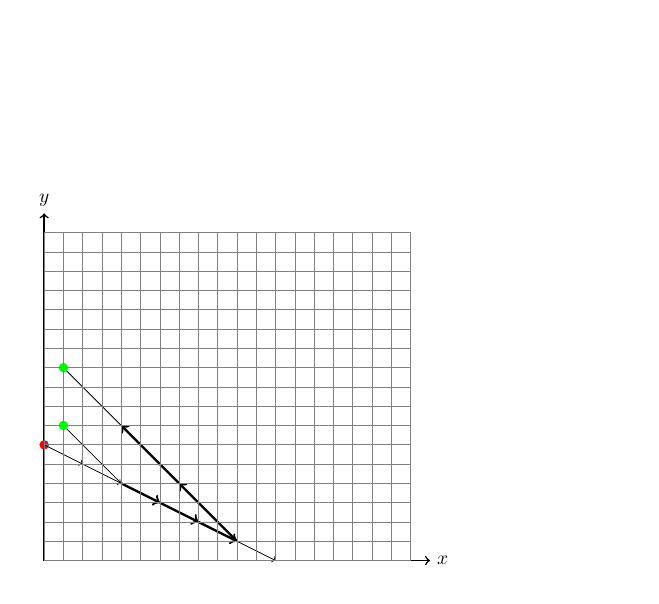
\begin{tikzpicture}[scale=0.35]
\scalebox{0.7}{
\draw[->, thick] (0, 0) -- (20, 0) node[right] {$x$};
\draw[->, thick] (0, 0) -- (0, 18) node[above] {$y$};

\fill[red] (0,6) circle (7pt);

\draw[->] (0,6) -> (2,5);
\draw[->] (2,5) -> (4,4);
\draw[very thick,->] (4,4) -> (6,3);
\draw[very thick,->] (6,3) -> (8,2);
\draw[very thick,->] (8,2) -> (10,1);
\draw[->] (10,1) -> (12,0);

\draw[->] (4,4) -> (1,7);
\fill[green] (1,7) circle (7pt);

\draw[very thick,->] (10,1) -> (7,4);
\draw[very thick,->] (7,4) -> (4,7);
\draw[->] (4,7) -> (1,10);
\fill[green] (1,10) circle (7pt);

\draw[step=1, gray, thin] (0, 0) grid (19, 17);
}
\end{tikzpicture}
\end{minipage}
\begin{minipage}{0.5\textwidth}
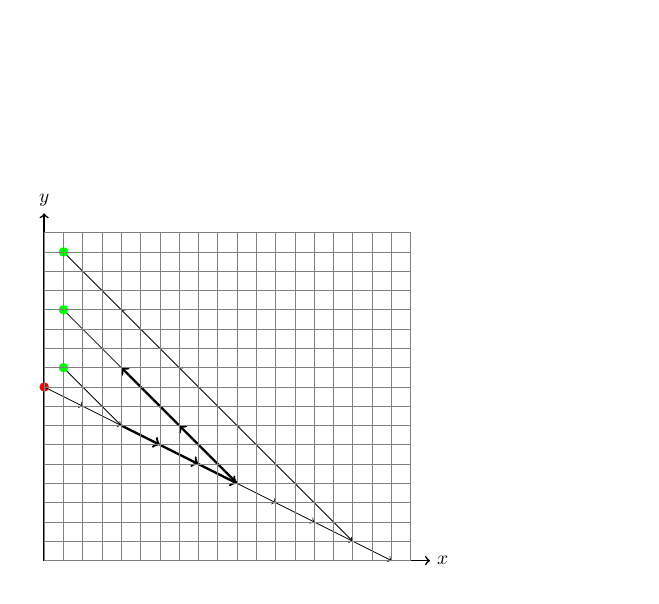
\begin{tikzpicture}[scale=0.35]
\scalebox{0.7}{
\draw[->, thick] (0, 0) -- (20, 0) node[right] {$x$};
\draw[->, thick] (0, 0) -- (0, 18) node[above] {$y$};

\fill[red] (0,9) circle (7pt);

\draw[->] (0,9) -> (2,8);
\draw[->] (2,8) -> (4,7);
\draw[very thick,->] (4,7) -> (6,6);
\draw[very thick,->] (6,6) -> (8,5);
\draw[very thick,->] (8,5) -> (10,4);
\draw[->] (10,4) -> (12,3);
\draw[->] (12,3) -> (14,2);
\draw[->] (14,2) -> (16,1);
\draw[->] (16,1) -> (18,0);

\draw[->] (4,7) -> (1,10);
\fill[green] (1,10) circle (7pt);

\draw[very thick,->] (10,4) -> (7,7);
\draw[very thick,->] (7,7) -> (4,10);
\draw[->] (4,10) -> (1,13);
\fill[green] (1,13) circle (7pt);

\draw[->] (16,1) -> (13,4);
\draw[->] (13,4) -> (10,7);
\draw[->] (10,7) -> (7,10);
\draw[->] (7,10) -> (4,13);
\draw[->] (4,13) -> (1,16);
\fill[green] (1,16) circle (7pt);

\draw[step=1, gray, thin] (0, 0) grid (19, 17);
}
\end{tikzpicture}
\end{minipage}

\caption{Left: $u_2 = 6$, $S_2 = \set{7,10}$. Right: $u_2 = 9$, $S_2 = \set{10,13,16}$.
Thick vectors add up to $p$.}
\label{fig:infix}
\end{figure}

Let $\alpha_1$ and $\alpha_2$ be empty sequences, $\eff(\beta_1) = (2, -1)$ and $\eff(\beta_2) = (-3, 3)$.
Let $u_1 = 0$, $v_1 = 1$. 
The set of solutions $(n_1, n_2)$ of~\eqref{eq:xy} is of the form $w+p^*$, where
$w = (2,1)$ and $p = (3,2)$, and
$\eff_2(p) = 3 \cdot (-1) + 2 \cdot 3 = 3$.
Figure~\ref{fig:infix} shows $R(u_2) = \set{7,10}$ when $u_2 = 6$, and $R(u_2)  = \set{10,13,16}$ when $u_2 = 9$.
In the latter case, elements of $R(u_2)$ correspond to the solutions $w$, $w+p$ and $w+2p$ of~\eqref{eq:xy},
i.e., to $w + kp$ for $k$ in an interval $[0,2]$.
According to Claim~\ref{cl:interval}, this is true in general.
%$S_2 = \setof{u + kp}{k\in I}$, for some interval $I$.
\end{example}

%The following claim states that the number of possible periods $p$ used in the run is an interval.

\begin{claim}\label{cl:interval}
For each $c \in S_1$ there exists an interval $I_{c} = [k_1, k_2]$, where $k_1\in \N$ and $k_2 \in \N_{\infty}$,
such that
$R(c) = \setof{\eff_2(w) + k \cdot \eff_2(p)}{k\in I_{c}}$.
% and path $\rho(b+kp)$ starting from $(b_1, c)$ is a valid if and only if $k \in I_c$. 
\end{claim}

\begin{proof}
It is sufficient to show that whenever $(u_1, c) \trans{w + k_1 \cdot p}$ and
$(u_1, c) \trans{w + k_2 \cdot p}$ for some
$k_1 < k_2 \in \N$,
then
$(u_1, c) \trans{w + k \cdot p}$ for all $k \in [k_1, k_2]$.
Fix $k \in [k_1, k_2]$.
Every point $x$ on the (possibly $\Z$-)path $(u_1, c) \trans{w + k \cdot p}$ is actually on a straight line between some two points,
one on the path $(u_1, c) \trans{w + k_1 \cdot p}$, and the other on the path $(u_1, c) \trans{w + k_2 \cdot p}$.
In consequence $x$, being a weighted average of the two points in $\N^2$, necessarily belongs to $\N^2$. 
Therefore $(u_1, c) \trans{w + k \cdot p}$ is a path.
\end{proof}

We notice that $\eff_2(p)$ can be negative, but this is irrelevant for our arguments.
%
By Claim~\ref{cl:interval}, for each $c \in S_1$ the set $R(c)$ is
is an arithmetic sequence of difference $\essdvass r := \absv{\eff_2(p)}$ and length equal to the cardinality
of the interval $I_{c}$.
%Thus $R(c) = b + (\essdvass r)^{\card{I_c}}$, for some $b\in\N$. 
Let $\spn(c)\in\N_\infty$ be the difference between the supremum of $R(c)$ and the minimal element in $R(c)$.
We say that $\spn(c) = \infty$ if $R(c)$ is infinite.
We split the proof into cases, depending on
whether $\essdvass r$ divides the difference $r$ of the sequence $S_1$, or not.
Additionally we have a case when $\essdvass r = 0$, in other cases we silently assume that $\essdvass r \neq 0$.


\para{Case I: $r$ is divisible by $\essdvass r$}

Therefore, if $\spn(c) \geq r$ then the sequence $R(c)$ actually touches the sequence $R(c+r)$,
i.e., their union is a larger arithmetic sequence of difference $\essdvass r$:

\begin{claim}\label{cl:merged}
If $R(c+r^*) \neq \emptyset$ and $c \geq D:= 3(M+r) \cdot M^2 + M \cdot \norm(w)$,
then $R(c+r^{\leq T}) = b+(\essdvass r)^{\leq T'}$ for some $b \leq c + \eff_2(w) + M \cdot \eff_2(p)$ and $T' \in \N_\infty$.
\end{claim}

\begin{proof}
We first show that $\spn(c) \geq r$.
Suppose $R(c+r^*) \neq \emptyset$ and $c \geq D$.
Due to the first assumption,  for some $n\in\N$ there is a path $(u_1, c+nr) \trans{(n_1, n_2)}$
of the form
\begin{align} \label{eq:Mp}
(u_1, c+nr) \trans{\alpha_1} (\essdvass{x}_1, \essdvass{y}_1) \trans{\beta_1^{n_1}} (\essdvass{x}_2, \essdvass{y}_2) \trans{\alpha_2} (\essdvass{x}_3, \essdvass{y}_3) \trans{\beta_2^{n_2}} (v_1, v_2).
\end{align}
In particular,  $u_1 \geq \drop_1(\alpha_1)$
and therefore $\essdvass x_1\geq 0$.
It is enough to take $(n_1, n_2) := w + Mp$ in \eqref{eq:Mp}.
Then $n_1 \geq M$, so $\essdvass x_2 \geq \essdvass x_1 + M \geq M \geq \drop_1(\alpha_2)$.
Therefore $\essdvass x_3\geq 0$.
Now we show that $c$ is large enough such that $(u_1, c) \trans{w+Mp}$ is nonnegative on the second coordinate as well.
As $\norm(p) \leq 2M$ then $n_1 + n_2 \leq M \cdot \norm(p) + \norm(w) \leq 2M^2 + \norm(w)$. Therefore
$\beta_1^{n_1}$ and $\beta_2^{n_2}$ can in total decrease the second coordinate by at most $M \cdot (2M^2 + \norm(w))$.
As $\alpha_1 + \alpha_2$ can in total decrease the second coordinate by at most $M$ and
$D \geq M + M \cdot (2M^2 + \norm(w))$ we conclude that indeed the path $(u_1, c) \trans{w+Mp}$ is valid.
For the same reasons, for every $m\in [M, M+r]$ there is a path $(u_1, c) \trans{w+mp}$, which guarantees $\spn(c) \geq r$. 

Now we use that fact that $\spn(c) \geq r$.
By monotonicity of \vass, if $R(c) = b+(\essdvass r)^{\leq {T'}}$
then $R(c+r)$ necessarily includes $R(c) + r= b+r+(\essdvass r)^{\leq {T'}}$.
Since $\spn(c) \geq r$, we have $b+r \in R(c)$, but also $b+r \in R(c+r)$,
and therefore the union $R(c) \cup R(c + r)$ forms one arithmetic sequence 
$b+(\essdvass r)^{\leq T'}$, for some $b\in\N$ and $T'$.
The similar reasoning applies to any finite union, namely to $R(c+r^{\leq m})$ for $m\in\N$.
In consequence, for every $T\in \N_\infty$ we have $R(c+r^{\leq T}) = b + (\essdvass r)^{\leq T'}$,
for some $b\in\N$ and $T'\in \N_\infty$,
and since $c+ \eff_2(w) + M \cdot \eff_2(p) \in R(c)$ we get the inequality $b \leq c + \eff_2(w) + M \cdot \eff_2(p)$, as required.
\end{proof}

We are ready for concluding Case I.
%Let $D = 3(M+r) \cdot M^2 + M \cdot \norm(w)$, as in the Claim~\ref{cl:bigspan}.
As $\norm(w) \leq \poly(B, M)$ we have $D \leq \poly(B, M, r)$.
We  partition $S_1 = a + r^{\leq T}$ into two subsets: $S'_1 = S_1 \cap [0,D)$
and $S''_1 = S_1 \cap [D,\infty)$, both being arithmetic sequences of difference $r$,
and consider $S'_1$ and $S''_1$ separately.
 
Concerning $S'_2:= R(S'_1)$,
as $\max(S'_1) \leq D$, all
elements of $S'_2$ are upper-bounded by a polynomial in $M$ and $r$, namely
$\max(S'_2) \leq M^2 \cdot (2M + D)$. 
Thus $S'_2$ can be seen as a finite sum of singletons, each of which
being an $(a', r', T')$-arithmetic sequence with $a' \leq M^2 \cdot (2M + D) \leq \poly(B,M,r)$,
$r' = 1$ and $T' = 0$. 
Clearly $r' = 1 \leq \poly(M)$, and hence $S'_2$ is of the required form.

Now we consider $S''_2:= R(S''_1)$.
If $S''_2 = \emptyset$ we are done.
Otherwise, let $c:= \min(S''_1)$.
Thus $S''_1 = c+r^{\leq T}$ for some $T \in \N_\infty$, 
and $D\leq c \leq \max(a, D+r)$.
%By Claim~\ref{cl:bigspan}, $\spn(c) \geq r$, and therefore using Claim~\ref{cl:neighbours} 
By Claim~\ref{cl:merged} we deduce that
$S''_2 = b + (\essdvass r)^{\leq T'}$ for some 
$b \leq c + \eff_2(w) + M \cdot \eff_2(p)$ and $T' \in \N_\infty'$. 
As $\eff_2(w) \leq \poly(B,M)$, $\eff_2(p) \leq \poly(M)$ and $c \leq a + \poly(B,M, r)$ we get $b \leq a + \poly(B, M, r)$.
We also have $\essdvass r \leq \poly(M)$, and hence
$S''_2$ is of the required form.


\para{Case II: $r$ is not divisible by $\essdvass r$}
%Assume now that $r$ does not divide $\eff_2(p)$. 

In that case we split $S_1 = a + r^{\leq T}$ into several
arithmetic sequences of difference $r \cdot \essdvass r$, namely into sequences of a form 
$(a + m \cdot r) + (r \cdot \essdvass r)^{\leq T'}$, where $m < \essdvass r$, 
and apply the above reasoning to each of this sequences separately. 
As $\essdvass r \leq \poly(M)$
we get also a finite set of arithmetic sequences with the base bounded by $a + \poly(B, M,r)$ and difference bounded by $\poly(M)$,
as required.

\para{Case III: $\essdvass r = 0$}
\Wlog we assume $R(S_1) \neq \emptyset$. For every $c \in S_1$ we have that either $R(c) = c + \eff_2(w)$ or $R(c) = \emptyset$. By monotonicity of VASS we have that if $R(c) \neq \emptyset$ then $R(c+r) \neq \emptyset$. Let $D := 3(M+r) \cdot M^2 + M \cdot \norm(w)$. Similarly as in the proof of Claim~\ref{cl:merged} we observe that if $c \geq D$ then for some $k \in N$ there is a run $(u_1, c) \trans{w+kp}$. Hence we have $R(S_1) = c + \eff_2(w) + r^{\leq T'}$ for some $T' \in \N_\infty$ and some $c \in S_1$ such that $c \leq \max(a, D+r)$. Therefore $R(S_1) = b + r^{\leq T'}$ for some $b \leq a + \poly(B,M,r)$ as required.

\end{proof}



%
%Observe, that if $(b_1, s) \trans \rho (b_2, t)$ for $s \in S_1$ and $t \in S_2$ then $x,y$ satisfy the following equation:
%$$\eff_1(\alpha_1\alpha_2) + x\eff_1(\beta_1) + y\eff_1(\beta_2) = b_2-b_1$$
%Hence we have that the set $S$ of such  pairs $(x,y)$ associated is included in set of solutions of the above equation, which can be represented by Lemma~\ref{lem:taming} as $L(B,P)$ for some sets $B, P \subseteq \N^2$ such that $\norm(B) \leq c(M+B)$ and $\norm(P) \leq cM$ for some constant $c \in \N_+$. We show, that $P$ has only one element $p$. This is because the set of solutions of the following equations over $\Q$ is one dimensional vector space and there is nonnegative solution, because of different signs of $\eff_1(\beta_1)$ and $\eff_1(\beta_2)$:
%$$x\eff_1(\beta_1) + y\eff_1(\beta_2) = 0$$
%Hence each path can be represented as $b+kp$ for some $k \in \N$ and $b \in B$ (recall that with each path we associated pair $(x,y)$). Because $B$ is finite and we are interested in a finite union representation it is enough to show that there exists polynomial $R(M)$ such that the set $S_2' =   \{y_2 \mid \exists_{y_1 \in S_1} (b_1, y_1) \trans{b+kp} (b_2, y_2), k \in \N \}$ is a finite union of $(a', r', T')$-arithmetic sets with $a' \leq a + (B+r) \cdot R(M)$ and
%$r' \leq R(M)$.
%
%We have $p=(p_1, p_2)$ and we write $\eff(p)$ for $\eff(\beta_1^{p_1}\beta_2^{p_2})$. Moreover $b = (b_1, b_2)$ and we write $\eff(b+kp)$ for $\eff(\alpha_1\beta_1^{b_1}\alpha_2\beta_2^{b_2}) + k \eff(p)$. First we solve a case when $|\eff_2(p)|$ divides $r$, to which we will reduce the other case. Let $m = \frac{r}{|\eff_2(p)|}$. Moreover, \mywlog we can assume that $S_2' \neq \emptyset$.
%The intuition is that the set $S_2'$ will be a condensing of $S_1$ due to repetitions of $p$ with base point $a'$ moved a bit. In order to conclude the prove we need a few claims. 
%\begin{claim}
%For each $s \in S_1$ there exists interval $I = [k_1, k_2]$ such that $k_1, k_2 \in \N_{\infty}$ and path $b+kp$ starting from $s$ is a valid path if and only if $k \in I$. 
%\end{claim}
%\begin{proof}
%It is enough to show, that if for $k_1 < k_2 \in \N$ we know, that $b+k_1p$ and $b+k_2p$ are valid paths starting from $s$ then for all $k_3 \in [k_1, k_2]$ we have that path $b+k_3p$ is a valid path starting from $s$. Let us fix $k_3 \in [k_1, k_2]$ and let $b=(b_1, b_2), p=(p_1, p_2) \in \N^2$. Recall, that $\eff(\beta_1) \in \N_+ \times \N_-$ and $\eff(\beta_2) \in \N_- \times \N_+$. Hence it is enough to show the following inequalities:
%$$\eff_1(\alpha_1\beta_1^{b_1+k_3p_1}\alpha_2\beta_2^{b_2+k_3p_2}) = \eff_1(\alpha_1\beta_1^{b_1+k_1p_1}\alpha_2\beta_2^{b_2+k_1p_2})$$
%$$\eff_2(\alpha_1\beta_1^{b_1+k_3p_1}) \geq \eff_2(\alpha_1\beta_1^{b_1+k_2p_1})$$
%For the first equality observe, that:
%\begin{align*}
%\eff_1(\alpha_1\beta_1^{b_1+k_3p_1}\alpha_2\beta_2^{b_2+k_3p_2}) & = \eff_1(\alpha_1\beta_1^{b_1+k_1p_1}\alpha_2\beta_2^{b_2+k_1p_2}) 
%+ (k_3-k_1)(p_1\eff_1(\beta_1) + p_2\eff_1(\beta_2)) \\
%& = \eff_1(\alpha_1\beta_1^{b_1+k_1p_1}\alpha_2\beta_2^{b_2+k_1p_2})
%\end{align*}
%The second inequality follows from the fact that:
%$$b_1+k_3p_1 \leq b_1+k_2p_1$$
%\end{proof}
%Let us by $I_x = [k_1^s, k_2^s]$ denote the interval for $x \in S_1$ and by $|I_x| = k_2^s - k_1^s$. Now we split elements of $S_1$ into three groups depending on the properties of the points in $S_1$.
%\begin{claim}\label{clm:split}
%For each $x \in S_1$ at least one of the following holds:
%\begin{itemize}
%\item $x \leq a + 3cM^2(B+r)$
%\item $x$ is the maximal element of $S_1$ and $[0,m] \subseteq I_x$
%\item $[0, m] \subseteq I_x$ and if $b+kp$ is executable from $(b_1,x)$ for $k > m$ than $b+(k-m)p$ is executable from $(b_1,x+m\eff_2(p))$ and $x+m\eff_2(p) \in S_1$. 
%\end{itemize}
%\end{claim}
%\begin{proof}
%Let us take $x \in S_1$ such that  $x > a + 3cM^2(B+r)$. Firstly, we show that $[0, m] \subseteq I_x$. Recall, that $\Lambda$ is one-turn and observe, that for all $k \in \N$ we have:
%$$\eff_1(\alpha_1\beta_1^{b_1}\alpha_2\beta_2^{b_2}) = \eff_1(\alpha_1\beta_1^{b_1}\alpha_2\beta_2^{b_2}) + k(p_1\eff_1(\beta_1) + p_2\eff_1(\beta_2))$$
%Hence, because $S_2$ is not empty we have that all paths $b+kp$ starting from $(b_1, x)$ are valid on the first counter. Hence we only need to deal with the second counter. Now observe, that for each $k \in [0,m]$ we have that maximal decrease of the second counter along path $b+kp$ is at most :
%\begin{align*}
%M + (b_1+kp_1)\eff_2(\beta_1) & \leq M + (c(M+B)+mcM)M \\
%& \leq 3cM^2(B+m) \leq 3CM^2(B+r) < x
%\end{align*}
%Hence $[0, m] \subseteq I_x$.
%If $x$ is the maximal element we are done. Otherwise,
%we show, that if $b+kp$ is executable from $(b_1,x)$ for $k > m$ than $b+(k-m)p$ is executable from $(b_1,x+m\eff_2(p))$ and $x+m\eff_2(p) \in S_1$. Observe, that $x+m\eff_2(p) = x+r$ if $\eff_2(p) > 0$ and $x+m\eff_2(p) = x-r$ otherwise. Because $S_1 =  a + r^{\leq K}$ and $x$ is not the maximal element of $S_1$ then in the first case $x+m\eff_2(p) \in S_1$. In the second case we have $x -  r \geq a+r-r \geq a$ and hence $x-r \in S_1$.
%
%Now it is left, that $b+(k-m)p$ is executable from $(b_1,x+m\eff_2(p))$. Similarly as before we only need to take care about the second counter. For this it is enough to observe, that:
%\begin{align*}
%x + m\eff_2(p) + \eff_2(\alpha_1\beta_1^{b_1+(k-m)p_1}) 
%& = x + \eff_2(\alpha_1\beta_1^{b_1+kp_1}) + mp_2\eff_2(\beta_2) \\
%& \geq x + \eff_2(\alpha_1\beta_1^{b_1+kp_1})
%\end{align*}
%This is due to $\eff_2(p) = p_1\eff_2(\beta_1) + p_2\eff_2(\beta_2)$ and $\eff_2(\beta_2) \geq 0$.
%Moreover:
%$$x+m\eff_2(p) \geq a+3cM^2(B+r)-r \geq a + M \geq |\eff_2(\alpha_1)|$$
%\end{proof}
%Now we can split $S_1$ into three parts $A_1, A_2, A_3$ such that elements from $A_1$ are the one with $s \leq a + 3cM^2(B+r)$, $A_3$ is the singleton or empty set containing the maximal element and $A_2$ is the rest of $S_1$. Observe, that $A_2 = a_2+r^{\leq K}$ for $a_2 \leq 3cM^2(B+r) + r, a_2 = a + kr$ for some $k \in \N$ and $K = T - k - 1$. Moreover observe, that if path start from $s \in A_2$ and is of the form $b+kp$ for $k > m$ than the same point is reachable from point $(b_1,s+m\eff_2(p))$ by path $b+(k-m)p$ due to Claim \ref{clm:split}. Hence, because we can iterate the argument at some point the starting point will be in $A_1 \cup A_3$ or $k \leq m$. Hence for points from $A_2$ we only need to consider paths $b+kp$ for $k \leq m$. Let us define $B_1, B_2$ and $B_3$.  
%$$B_1 = \bigcup_{x \in A_1, k \in I_x} \set{x + \eff_2(b+kp)}$$
%$$B_2 = \bigcup_{x \in A_2, k \in [0,m]} \set{x + \eff_2(b+kp)} 
%= a_2 + r^{\leq T} + \eff_2(b) + \eff_2(p)^{\leq m}$$
%$$B_3 = \bigcup_{x \in A_3, k \in I_s} \set{x + \eff_2(b+kp)}$$ 
%Which if $A_3 \neq \emptyset$ can be represented as
%$$B_3= a + (T+1)r  + \eff_2(b) + \eff_2(p)^{\leq |I_{x_{max}}|}$$
%where $x_{max}$ is the element of $A_3$. From now on we fix this maximal element and put $|I_{x_max}| = 0$ if it does not exist. 
%Let us observe:
%$$S_2 = B_1 \cup B_2 \cup B_3$$
%We deal separately with $B_1$ and $B_2 \cup B_3$. Because $a_2 + \eff_2(b) \leq 3cM^2(B+r) + r $ clearly, in order to show, that $B_2 \cup B_3$ is  of the form we want it is enough to show the following claim (recall that $\eff_2(p)$ can not be zero due to divisibility condition):
%\begin{claim}
%$(B_2 \cup B_3) \cap [a_2 + \eff_2(b), \infty] = a_2 + \eff_2(b) + |\eff_2(p)|^{\leq T'}$ where $T' = m(T+1) + |I_{x_{max}}|$ if $\eff_2(p) > 0$ and $T' = m(T+1)$ if $\eff_2(p) < 0$ .  
%\end{claim}
%\begin{proof}
%Firstly we show $(B_2 \cup B_3) \cap [a_2 + \eff_2(b), \infty] \subseteq a_2 + \eff_2(b) + |\eff_2(p)|^{\leq T'}$. Let us take any $x \in (B_2 \cup B_3) \cap [a_2 + \eff_2(b), \infty]$. The first case is that $x \in B_2$ and hence 
%$$x = a_2 + \eff_2(b) + k_1r + k_2\eff_2(p)$$
%for $k_1 \leq T$ and $k_2 \leq m$. We have 
%$$x = a_2 + \eff_2(b) + k_1m|\eff_2(p)| + k_2\eff_2(p)$$
%and hence if $\eff_2(p) > 0$ we have 
%$$x = a_2 + \eff_2(b) + (k_1m + k_2)|\eff_2(p)| \in a_2 + \eff_2(b) + |\eff_2(p)|^{\leq T'}$$
%and if $\eff_2(p) < 0$ we have 
%$$x =  a_2 + \eff_2(b) + |\eff_2(p)|^{k_1m-k_2}$$
%Because $x \geq a_2 + \eff_2(b)$ we have $k_1m-k_2 \geq 0$ and hence $x \in a_2 + \eff_2(b) + |\eff_2(p)|^{\leq T'}$ .
%
%Now we show $a_2 + \eff_2(b) + |\eff_2(p)|^{\leq T'} \subseteq (B_2 \cup B_3) \cap [a_2 + \eff_2(b), \infty]$. Let us take $x = a_2 + \eff_2(b) + k|\eff_2(p)|$ for some $k \leq T'$. Firstly let us consider case when $\eff_2(p) > 0$. 
%\begin{align*}
%x & = a_2 + \eff_2(b) + \floor{\frac{k}{m}}m|\eff_2(p)|+ (k\mod m)|\eff_2(p)| \\
%& = a_2 + \eff_2(b) + \floor{\frac{k}{m}}r + (k \mod m)\eff_2(p)
%\end{align*}
%Observe, that if $k \leq m(T+1)$ we have
%$$\floor{\frac{k}{m}} \leq \floor{\frac{m(T+1)}{m}} = T+1$$
%Hence $x \in a_2 + \eff_2(b) + r^{\leq T} + |\eff_2(p)|^{\leq m} = B_2$
%If $k > m(T+1)$ then observe, that $k - m(T+1) \leq |I_{x_{max}}|$ and see, that
%$$x = a_2 + \eff_2(b) + r(T+1) + \eff_2(p)^{k-m(T+1)} \in B_3 $$
%
%Now we consider case when $\eff_2(p) < 0$. Then:
%$$x=a_2 + \eff_2(b) + \ceil{\frac{k}{m}}m|\eff_2(p)|-(m - (k \mod m))|\eff_2(p)|$$
%Then if $k \leq mT$ we have:
%$$x \in a_2 + \eff_2(b) + r^{\leq T}+\eff_2(p)^{\leq m} = B_2 $$
%And if $k > mT$ we have:
%$$x \in a_2 + \eff_2(b) + (T+1)r + \eff_2(p)^{\leq m} \subseteq B_3$$
%
%\end{proof}
%For the set $B_1$ it is enough to prove the following Claim:
%\begin{claim}
%$B_1$ can be represented as a finite union of $(a', r',T')$-arithmetic sets with $a' \leq a + 10cM^4(B+r)$ and $r' \leq cM$.
%\end{claim}
%\begin{proof}
%The first case is that the second counter is at most $3cM^2(B+r)$ at the beginning. The first counter is at most $B$ at the beginning. Then after $\alpha_1$ they are at most $3cM^2(B+r) + M \leq 4cM^2(B+r)$. Then after all execution of the $\beta_1$ the sum of the counters is at most $8cM^3(B+r)$ then after $\alpha_2$ the sum of counters is at most $8cM^3(B+r) + 2M$ and finally after the last execution of $\beta_2$ the sum of counters and hence also the second counter is at most $8cM^4(B+r) + 2M^2 \leq 10cM^4(B+r)$ as needed. Hence there is a finite number of such elements and they can be represented as a singleton arithmetic sets.
%The second case is that the second counter is at least $3cM^2(B+r)$ at the beginning. Let the beginning point be $x$. We show, that elements of $B_1$ obtained by the paths starting in $x$ can be represented as an arithmetic-set. Therefore assume this set is not empty (otherwise it is trivial). Recall, that $\Lambda$ is one-turn and observe, that for all $k \in \N$ we have:
%$$\eff_1(\alpha_1\beta_1^{b_1}\alpha_2\beta_2^{b_2}) = \eff_1(\alpha_1\beta_1^{b_1}\alpha_2\beta_2^{b_2}) + k(p_1\eff_1(\beta_1) + p_2\eff_1(\beta_2))$$
%All paths $b+kp$ starting from $x$ are valid on the first counter. Hence we only need to deal with the second counter. Now observe, that  we have that maximal decrease of the second counter along path $b$ is at most :
%$$M + b_1\eff_2(\beta_1) \leq M + c(M+B)M \leq 3cM^2B$$ Hence path $b$ is also valid on the second counter. Hence $x_2 + \eff_2(b) \in B_1$ and $x_2 + \eff_2(b) \leq a + 3cM^2(B+r) + \eff_2(\alpha_1\alpha_2) + b_1\eff_2(\beta_1) + b_2\eff_2(\beta_2) \leq a + 3cM^2(B+r) + M +  2c(M+B)M \leq a + 10cM^2(B+r)$. Now if $\eff_2(p) > 0$ then the set can be represented as $(x_2 + \eff_2(b), \eff_2(p), T')$-arithmetic set, which satisfies the conditions. Otherwise all elements are at most $a + 10cM^2(B+r)$ and can be represented as singleton arithmetic sets, which satisfies the conditions.
%\end{proof}
%By previous claims we know, that $S_2$ is a finite union of $(a',r', T')$-arithmetic sets for $a' \leq a + 10cM^4(B+r)$ and $r' \leq cM$.
%
%
%Now we come back to the case when $r$ is not divisible by $|\eff_2(p)|$. The first subcase is that $\eff_2(p) = 0$. Then all paths $b+kp$ have the same effect so we only need to consider path $b$. The lowest $x \in S_1$ from which the path $b$ is executable is at most $M + b_1\eff_2(\beta_1) + a + r \leq M + c(M+B)M + a+r \leq a + 3M^2(B+r)$. Hence set $S_2$ can be represented as $(a', r, T')$-arithmetic set for $a' \leq a+ 3M^2(B+r) + \eff_2(b) \leq a+ 3M^2(B+r) + M+2c(M+B)M \leq a + 10M^2(B+r)$. The second subcase is that $\eff_2(p) \neq 0$. Then we can split $S_1$ into several $(a'', \eff_2(p)r, T'')$-arithmetic sets with $a'' \leq a + \eff_2(p)r \leq a + (2cM^2+M)r$ then we can apply the first case and get representation of $S_2$ as a finite union of $(a',r', T')$-arithmetic sets with $r' \leq cM$ and $a' \leq a + (2cM^2+M)r + 10cM^4(B+r) \leq a+ 13M^4(B+r)$. Thus by setting $R(M) = 13cM^4$ we conclude the proof. 
%\end{proof}



\begin{proof}[Proof of Claim~\ref{cl:suffix}]
\Wlog we assume $\Lambda = \alpha_1\beta_1^*\alpha_2\beta_2^*\alpha_3\beta_3^*\alpha_4$.
Let $S_1 = b + \set{p}^{\leq T}$  and $S_2 = \reach_{\Lambda}(S_1)$. Recall, that $\eff_j(\gamma)$ denotes the $j$-th coordinate of $\eff(\gamma)$, and
$\drop_j(\gamma)\in\N$ is the maximal value of $-\eff_j(\delta)$, where $\delta$ ranges over prefixes of $\gamma$,
that is  the maximal amount by which the $j$-th coordinate can be decreased along $\gamma$.

Similarly as in the proof of Claim~\ref{cl:prefix} we describe paths $s = (s_1,s_2) \tran (t_1, t_2) = t$ in $\Lambda$,
\begin{align*}
(s_1, s_2) = &
(a_1^1, a_2^1) \trans{\alpha_1} (b_1^1, b_2^1) \trans{\beta_1^{n_1}}
(a_1^2, a_2^2) \trans{\alpha_2} (b_1^2, b_2^2) \trans{\beta_2^{n_2}} \\
& (a_1^3, a_2^3) \trans{\alpha_3} (b_1^3, b_2^3) \trans{\beta_3^{n_3}}
(a_1^4, a_2^4) \trans{\alpha_4} (b_1^4, b_2^4) = (t_1, t_2).
\end{align*}
Notice that $(s_1, s_2) = (a_1^1, a_2^1) \in S_1$, so $(a_1^1, a_2^1) = u + p^n$ for some $n \in \N$. The following system of linear Diophantine inequalities $\U$ with unknowns $a_1^i, a_2^i, b_1^i, b_2^i$ for $i \in [1,4]$, and $n_i$, for $i \in [1,3]$, and unknown $n$, ensures that the effects of $\alpha_i$ and $\beta_i^{n_i}$ are respected, and that all points along $\alpha_i$ remain nonnegative and that $s \in S_1$:

\begin{align*}
a^{i}_j + \eff_j(\alpha_i) \ = \ & \ b^{i}_j  & a^1_j \ = \ & \ u_j + n \cdot p_j \\
b^{i}_j + n_i \cdot \eff_j(\beta_i) \ = \ & \ a^{i+1}_j & n \ \leq \ & \ T \label{eq:LPS_bound} \\
a^i_j - \drop_j(\alpha_i) \ \geq \ & \ 0 
\end{align*}
Notice that each $\beta_i$ is a single transition, so nonnegativity of $(b_i^1, b_i^2)$ and $(a_{i+1}^1, a_{i+1}^2)$
implies that all the vectors along  $\beta_i^{n_i}$ are also nonnegative. Therefore, we do not need to
add an analog of $a^i_j - \drop_j(\alpha_i) \geq 0$ for $\beta_i$ to the above system. We first focus on the solutions of $\U$ without the equation $n \leq T$, 
and inequalities $a^i_j - \drop_j(\alpha_i) \geq 0$ transformed into equations with dummy variables on the right, similarly as in the proof of Claim~\ref{cl:prefix}. Let us call such system $\U'$. All the coefficients of $\U'$ are bounded by $\max(M, \norm(u), \norm(p))$. By Lemma~\ref{lem:solutions} set of solutions of $\U'$ can be described as $L(U, V)$ for $\norm(U \cup V) \leq \poly(M, \norm(u), \norm(p))$.

%$\norm(U \cup P) \leq R(N) \cdot R(M)$ for some polynomial $R$. After adding equalities~\eqref{eq:LPS_end2} by Proposition~\ref{prop:fix_variables} we get solutions of the form $L(U', P')$ for $\norm(U') \leq R(N) \cdot R(M) \cdot (\norm(b_1) + 1)$ and $\norm(P') \leq R(N) \cdot R(M)$.

Now we have to care about the last inequality, namely $n \leq T$. If for some $a \in U$ we have $n > T$ then we can remove it from $U$. Let $U'$ be the set $U$ without the removed elements.
As the set $U'$ is finite it is enough to prove the conclusion of Claim~\ref{cl:suffix} separately for each $a \in U'$. Fix $a \in U'$.
We have $\norm(a), \norm(V) \leq \poly(M, \norm(u), \norm(p))$.
It is enough to prove that elements of the set $L(a, V)$ that additionally satisfy $n \leq T$, projected to the variables
$b^4_1$ and $b^4_2$ can be described as a finite union of the sets of the form we need.

Let us consider all the elements of set $V$. Let $Q \subseteq V$ be the set of these elements $v \in V$,
for which $v[n] = 0$ (that means that unknown $n$ is equal to $0$ in elements $v$),
while $P = V \setminus Q$ be the set of the other elements $v \in V$,
so that for which $v[n] > 0$.
Notice that using elements in $Q$ does not influence satisfying $n \leq T$, therefore they
can be used unbounded number of times.
Let $P = \set{p_1, \ldots, p_\ell}$ and let $p_i[n] = c_i$. For each $x \in L(a, V)$ we have $x = a + q + \Sigma_{i=1}^{\ell}k_i \cdot p_i$ where $q \in Q^*$. Hence, in order to satisfy $n \leq T$ we have to satisfy $\innprod c k \leq (T - a[n])$, where $c = (c_1, \ldots, c_\ell) \in \N_{>0}^\ell$ and $k = (k_1, \ldots, k_\ell) \in \N^\ell$.
As $c \in \N_{>0}^\ell$, if $T - a[n] < 0$ then the set of solutions is empty. Otherwise, the set of solutions can be represented as $a+P^{c \cdot x \leq T - a[n]}+Q^*$. Recall that $\norm(a), \norm(P \cup Q) \leq \poly(M, \norm(u), \norm(p))$, and additionally $c \in \N_{>0}^{\ell}$. Additionally $\norm(c) \leq \ell \cdot \norm(P)$, where
$\ell$ is the number of elements in $P$, thus $\ell \leq (\norm(P) + 1)^k$, where $k$ is the number of unknowns in $\mathcal U$
(so $k$ is a constant).
In consequence $\norm(c) \leq \poly(M, \norm(u), \norm(p))$. Summarising, the projection
of $a+P^{c \cdot x \leq T - a[n]}+Q^*$ into variables $b^4_1$ and $b^4_2$ is of the required form.
\end{proof}
%
Claims \ref{cl:prefix}, \ref{cl:infix} and \ref{cl:suffix} are thus shown, and hence so is Lemma~\ref{lem:sandwich-raw}.
%
\end{appendixproof}


In the proof of Lemma~\ref{lem:main} we actually need polynomial approximability not only for \dvass, but also for
its generalisation, \geomvass. It is stated below and shown in the Appendix using Lemma~\ref{lem:2vass-sandwich}

\begin{lemma} \label{lem:geom-sandwich}
\Geomvass are \sandwich.
\end{lemma}
%
\begin{appendixproof}[Proof of Lemma~\ref{lem:geom-sandwich}]
Fix an arbitrary \geomvass $(V, s)$ and let $M = \size(V,s)$.
Norms of vectors generating $\cone V$ --- i.e., effects of simple cycles --- are at most $M$, 
as no transition repeats along a simple cycle.
The effect $\delta \in \Z^3$  of each simple cycle
satisfies $\innprod a \delta = 0$, where $a\in\Z^3$ is a vector orthogonal to $\Lin V$,
or equivalently, orthogonal to some two effects of simple cycles.
The vector $a$ is thus an integer solution of a system of 2 linear equations with 3 unknowns,
where absolute values of coefficients are bounded by $M$.
By Lemma \ref{lem:taming}, there is such an integer solution 
$a=(a_1, a_2, a_3)$ with $\norm(a)\leq D=\OO(M^2)$.


In consequence, on every path $s \tran t$ the value of inner product with $a$ is bounded polynomially
with respect to $M$:
%
\begin{claim} \label{claim:axx}
Every configuration $q(x)\in \reach(V,s)$  satisfies
$-C \leq \innprod a x \leq C$, where $C = \OO(M\cdot D)$. 
\end{claim}
%

We rely on the construction of \cite[Lemma 5.1]{Zhang-geom}, which transforms a 
\geomvass $(V,s )$ into a \dvass $(\essdvass V, \essdvass s)$ of size at most $R(M)$
for some polynomial $R$, by dropping on of dimensions of $V$.

\para{Case I: $a$ contains both positive and negative numbers}
\Wlog assume that $a_1, a_2 \geq 0$ and $a_3<0$,
in which case it is the third coordinate which is dropped 
by the construction of \cite[Lemma 5.1]{Zhang-geom}.
States of $\essdvass V$ are of the form $\pair q c$, where $q\in Q$ and $c\in\setfromto {-C} C$, 
plus some further auxiliary states, omitted here.
Due to Claim \ref{claim:axx},
there is a one-to-one correspondence between
reachable configurations in $V$ and reachable configurations in $\essdvass V$:
\[
e = q(x_1, x_2, x_3) \quad \longmapsto \quad
\essdvass e = \pair q c(x_1, x_2), 
\qquad
\text{ where } c = \innprod a x.
\]
%
The tight correspondence between paths of $V$ and $\essdvass V$,
 given in Claim \ref{claim:V321} below, is essentially 
Lemma 5.1 of \cite{Zhang-geom}:
%
\begin{claim} \label{claim:V321}
For every configurations $s,u$,
here is a path $s \tran u$ in $\essdvass V$
if, and only if,
there is a path $\essdvass s \tran \essdvass u$ in $\essdvass V$.
\end{claim}
%
By Lemma \ref{lem:2vass-sandwich}, there is a polynomial $F$ such that 
for every $B\in\N$,
in the \dvass
$(\essdvass V, \essdvass s)$ obtained by the above construction, 
for every its state $\pair q c$, the set 
$\reach_{\pair q c}(\essdvass V, \essdvass s)$ is \kanapka {$F(M')$} {$B$}, where
$M'=\size(\essdvass V, \essdvass s) \leq R(M)$, and hence also
\kanapka {$F(R(M))$} {$B$}.
We claim that for every state $q\in Q$, for every $B\in\N$, 
the set $\reach_q(V,s)$ is \kanapka {$G(F(R(M)))$} {$B$}, for some nondecreasing polynomial $G$.
Indeed, for any $B\in\N$, any ($B$-approximation of) a linear set 
$L = w + P^*\subseteq \N^2$, where $w=(w_1, w_2)$, witnessing that
$\reach_{\pair q c}(\essdvass V,\essdvass s)$  is \kanapka {$F(R(M))$} {$B$}
is transformed to a ($B$-approximation of) linear set $L'$ witnessing that
$\reach_{q}(V,s)$  is \kanapka {$G(F(R(M)))$} {$B$}, as follows.
Take as base the unique vector $w'=(w_1, w_2, w_3)$ such that $a_1 w_1 + a_2 w_2 + a_3 w_3 = c$.
For every period $p=(p_1, p_2) \in P$, take into the set $P'$  the unique vector
$p'=(p_1, p_2, p_3)$ such that $a_1 p_1 + a_2 p_2 + a_3 p_3 = 0$.
Since $a_3>0$, it is guaranteed that $p_3 \geq 0$, and therefore $p'\in\N^3$.
Let the polynomial $G$ bound the blowup of $\norm(b')$ with respect to $\norm(b)$, and 
$\norm(p')$ with respect to $\norm(p)$, for instance
$G(x) = M \cdot x + B$.
The union of all ($B$-approximations of) 
so described sets $L' = w' + (P')^*$, for all $c\in\setfromto {-C} C$, provides the witness that
$\reach_{q}(V,s)$ is \kanapka {$G(F(R(M)))$} {$B$}.

\para{Case II: $a$ is non-negative or non-positive}
\Wlog assume $a\geq \vec 0$ and $a_3 > 0$.
By Claim \ref{claim:axx}, for each $q(x) \in \reach(V,s)$
we thus have $x_3 \leq C$.
%
We transform $(V,s)$ into $(\essdvass V, \essdvass s)$ 
with states of the form $\pair q c$, where $q\in Q$ and $c\in\setfromto {0} C$, 
by storing the third coordinate in state:
\[
e = q(x_1, x_2, x_3) \quad \longmapsto \quad
\essdvass e = \pair q c(x_1, x_2), 
\qquad
\text{ where } c = x_3.
\]
As above, $\size(\essdvass V, \essdvass s) \leq R(M)$, for a polynomial $R$.
The argument  that for every $B\in\N$,
the set $\reach_{q}(V,s)$ is \kanapka {$G(F(R(M)))$} {$B$}, is similar to Case I (but simpler).
\end{appendixproof}

%
%\begin{lemma} \label{lem:nondiag-sandwich}
%Non-forward-diagonal lollypop \tvass are \sandwich.
%%\slawek{uwaga na $\norm(a) \leq 2R(M) \cdot B$}
%\end{lemma}
%%
%%\begin{proof}
%\begin{proof}[Proof of Lemma \ref{lem:nondiag-sandwich}]
%%\slawek{could go to appendix}
%Exactly as in Case 3 of the proof of Lemma \ref{lem:1comp}, one can transform
%a non-forward-diagonal lollypop \tvass $(V, s)$ into
%three \geomvass $(V_1, s_1), (V_2, s_2), (V_3, s_3)$.
%In each configuration of the three \dvass, the value of the
%missing coordinate is determined by state.
%By Claim \ref{claim:nondiag2vass}, the lengths of paths in $V$ are the same as (jointly) the 
%paths in the three \geomvass, and
%by Claim \ref{claim:nondiagsize} the size of each $(V_j, s_j)$  is bounded by
%$R(M)$, where $M = \size(V,s)$.
%The blowup of the transformation is thus bounded by a nondecreasing polynomial $R$.
%We combine the transformation with Lemma \ref{lem:geom-sandwich},
%according to which there is a nondecreasing polynomial $F$
%such that the class of \geomvass is \parsandwich{$F$},
%to deduce that
%the class of non-forward-diagonal 1-component \tvass is \parsandwich{$(F(R(\_))$}.
%Indeed, all ($B$-approximations of) linear sets witnessing that
%$\reach_{\pair q b}(s_j)$ in $V_j$ is \kanapka {$F(R(M))$} {$B$}, fro all $b$ and $j$,
%jointly witness that
%$\reach_{q}(s)$ in $V$ 
%is \kanapka {$F(R(M))$} {$B$}.
%%by adding the missing coordinate as follows:
%%add the missing coordinate in the base vector $b$ as determined by the target state $q$;
%%and in each period vector $v\in P$, add the missing coordinate 0.
%%\end{proof}
%\end{proof}
%


\section{A New Framework}
The formulated critiques articulate that a better formulation of evaluation criteria for obfuscating transformations is needed to provide better guidance on how to assess their real strengths and weaknesses rather than reporting artificial, irrelevant, or even misguided proxies. The primary aim of such guidance is to help researchers maximize the impact of their work by convincing other researchers that they can build on this work for their own research and by convincing practitioners of the relevance of the work for real-world software protection. To a large degree, such impact depends on the validity of the performed evaluations. This includes the commonly used criteria of validity in software engineering, such as construct, conclusion, internal, and external validity~\cite{Wohlin} but also less commonly considered criteria such as instantiation validity~\cite{lukyanenko2014instantiation}. \emph{Reducing such threats to validity is the aim of this framework.} 

In line with many of the existing definitions discussed in Sections~\ref{sec:collberg_nagra_def},~\ref{sec:completeness}, and~\ref{sec:adequacy}; in line much of the examples mentioned in Section~\ref{sec:attack_tool_examples}; and in line with the recommendations of De Sutter et al.~\cite{desutter2024evaluation} that evaluations obfuscation strength evaluations should be based on their impact on real-world attacks, we put forward that the used evaluation criteria should be based on specific program properties that adversaries can target with specific attack strategies, and on the impact that the obfuscations have on those strategies. 

Unlike NC, we think that a concept similar to resilience needs to be a core criterion. And unlike the research on AI-based potency, we feel the criteria need to be practical, e.g., in the sense that they are consistent with the fact that MATE attackers can always reveal the properties they are after, and that the required effort of a whole attack strategy, not only of individual steps, is what matters. Unlike existing evaluation criteria defined in terms of analysis, we define them in terms of attack strategies, which consist of different categories of attacks steps being executed: 
\begin{enumerate}
\item knowledge gathering, i.e., revealing properties:
\begin{enumerate}
    \item revealing static/dynamic artifacts in the program;
    \item revealing relations between artifacts;
    \item revealing features of the artifacts and the relations;
    \item assigning priorities to artifacts and relations; 
    \item revealing mappings between abstract artifacts, properties, and relations; and concrete ones.
\end{enumerate}
\item artifact manipulation, such as lifting a code fragment from a program for ex situ execution, tampering with a SP to undo it, or altering its execution state to bypass a SP; 
\item decision making on the next steps to execute based on the determined priorities and already gathered knowledge.
\end{enumerate}
These categories capture the four goals of analyses in the survey by Schrittwieser et al.\ on obfuscation vs.\ program analysis~\cite{survey2016}, the activities modeled by the reverse engineering formalization by Faingnaert et al.~\cite{checkmate24}, the activities observed in experiments by Ceccato et al.~\cite{emse2019}, in a survey on the practice of malware analysis~\cite{wong2021inside}, etc. For example, code comprehension tasks, such as understanding that some code fragment implements a quicksort, are instantiated by combinations of (1a), (1b), (1c), and (1e). The same holds for making hypotheses, confirming them, and discarding them, which are important attack activities as observed by Ceccato et al.~\cite{emse2019}. Finding the location of relevant code and data in a program in addition requires (1d) to classify the revealed information into relevant vs.\ irrelevant ones. Undoing an obfuscation obviously requires (2). 

\emph{It is hence against combinations of these kinds of attack steps, and the possible methods to execute them in relevant attack strategies, that obfuscations can and should be evaluated.}

Importantly, the methods used to execute these steps can be unsound and non-conservative. For example, trace-based analysis techniques to reveal properties are unsound. Artifact manipulation may be non-conservative when the applied transformation does not conserve the behavior under all possible circumstances. When some hypothesis is being made by an adversary in some attack steps that are not confirmed in later steps, for example because the adversary reaches their goal first, the steps building on that hypothesis are obviously unsound as well. 

Given the wide range of properties that adversaries might be interested in, and the wide range of analyses techniques that can help them, it makes no sense to propose a one-size-fits-all set of evaluation metrics or to prescribe exactly what metrics should be measured. We hence limit ourselves to prescribing which criteria should be evaluated, aiming at defining them in ways that avoid the confusion that has existed regarding previous definitions. Our new framework of criteria includes relevance, effectiveness (and its poor man's alternative of efficacy), robustness, concealment, stubbornness, sensitivity, predictability, and cost. Table~\ref{tab:criteria} lists them all, including their subcriteria. 

\begin{table}[t]
    \centering
    \begin{tabular}{c p{6cm} l}
\hline
    \multicolumn{3}{l}{\textbf{Relevance}}\\
%    \midrule
       & Attack Steps Relevance  & $Re_{a}$ \\
       & Program Property Relevance & $Re_{p}$ \\
       & Obfuscation Impact Relevance & $Re_{o}$ \\
       & Metrics Relevance & $Re_{m}$ \\
       & Tool Availability:& $Re_{t}$ \\
       & Sample Relevance & $Re_{s}$\\
       & Layered Protection Relevance & $Re_{l}$\\
%   \midrule
    \multicolumn{3}{l}{\textbf{Effectiveness}}\\
   & Isolated Outcome Effectivness & $E_{o,i}$ \\
   & Marginal Outcome Effectivness & $E_{o,m}$ \\   
   & Isolated Resource Effectivness & $E_{r,i}$ \\
   & Marginal Resource Effectivness & $E_{r,m}$ \\
%      \midrule
    \multicolumn{3}{l}{\textbf{Robustness}}\\
     &  Isolated Outcome Delta & $Ro_{o,i}$ \\
     &  Marginal Outcome Delta & $Ro_{o,m}$ \\
     &  Isolated Resource Delta & $Ro_{r,i}$ \\
     &  Marginal Resource Delta & $Ro_{r,m}$ \\
     &  Deployment Delta & $Rd_{o,m}$ \\
%           \midrule
    \multicolumn{3}{l}{\textbf{Concealment}}\\
         &  Local Concealment & $C_{l}$ \\
         &  Global Concealment & $C_{g}$ \\
         &  Strategic Concealment & $C_{s}$ \\
    \multicolumn{3}{l}{\textbf{Stubbornness}}\\
         &  Outcome Stubbornness & $St_{o}$ \\
         &  Resource Stubbornness & $St_{d}$ \\
   \multicolumn{3}{l}{\textbf{Sensitivity}}\\
         &  Sample Feature Sensitivity & $Se_{s}$ \\
         &  Attack Instantiation Sensitivity & $Se_{a}$ \\       
         &  Protection Instantiation Sensitivity & $Se_{pi}$ \\       
         &  Protection Configuration Sensitivity & $Se_{pc}$ \\       
         &  Build Tool Flow Sensitivity & $Se_{b}$ \\                
         &  Platform Sensitivity & $Se_{p}$ \\ 
   \multicolumn{3}{l}{\textbf{Predictability}}\\
         &  Sample Feature Predictability & $P_{s}$ \\
         &  Attack Instantiation Predictability & $P_{a}$ \\       
         &  Protection Instantiation Predictability & $P_{pi}$ \\       
         &  Protection Configuration Predictability & $P_{pc}$ \\       
         &  Build Tool Flow Predictability & $P_{b}$ \\                
         &  Platform Predictability & $P_{p}$ \\ 
   \multicolumn{3}{l}{\textbf{Cost}}\\
         &  Performance Cost & $C_{p}$ \\
         &  SDLC Cost & $C_{sdlc}$ \\       
         \hline
    \end{tabular}
    \caption{All obfuscation evaluation criteria and subcriteria}
    \label{tab:criteria}
\end{table}


\subsection{Relevance of the Evaluation Constructs}
The first criterion to be considered in an evaluation of an obfuscation's strength is the relevance of all the constructs used in the evaluation. To maximize the relevance of a researcher's evaluation results for practitioners, the used constructs need to representative for real-world software protection. 


Researchers, however, face deadlines and budget and resource limitations. Different researchers therefore aim for different technology readiness levels (TRLs) with their research. That is obviously fine, and different criteria of our framework support research and evaluations at the various levels, while at the same time enabling and encouraging the researchers to be transparent about the TRL of their research results. Ensuring this transparency, and forcing the researcher to reason about the impact of evaluation methodology choices on the relevance of the evaluation results and their validity is the aim of the seven relevance criteria detailed below. 

It should come as no surprise that we first focus on criteria that pertain more to the evaluation method than to the obfuscation being evaluated itself. The reason is of course the lack of standardization in the domain of SP~\cite{Basile23}. Where certification has been standardized (e.g., smart card security~\cite{common_criteria}) and where risk management standards have been adopted (e.g., NIST SP 800-39~\cite{nistSP800-39} in network security~\cite{Gartner-report-riskanalysis}), concise evaluation results can be published that refer to those standards so that all stakeholders know how to interpret those results. In MATE SP, on the contrary, only some embryonic steps toward standardization have been proposed~\cite{Basile23}. Lacking standardized evaluation methods, evaluation results are meaningless without proper framing. 

An evaluation therefore stands or falls with accurate and complete framing, which can be achieved by assessing the evaluation according to the seven relevance criteria we put forward:

\paragraph{$Re_a$ - Attack Steps Relevance:} To what extent are the considered attack step combinations relevant? In which relevant attack strategies are they used, meaning attack strategies with a proven track record in the scientific literature or in real-world reporting? Are there no alternative combinations known that can produce the same results as the considered ones but are simpler to execute? Is the starting point of the considered attack steps realistic, i.e., the preceding attack steps? Does the evaluation use realistic outputs of those preceding steps as inputs to evaluate the considered attack step combination?

\paragraph{$Re_p$ - Program Property Relevance:} To what extent are the program properties relevant that the protection is supposed to hide, and that adversaries supposedly want to reveal through the considered attack steps? Are there alternative strategies with which adversaries can reach the same end goal, but without requiring them to obtain the results of the considered attack steps, i.e., without them requiring to reveal exactly those program properties?

\paragraph{$Re_o$ - Obfuscation Impact Relevance:} To what extent does the impact of the evaluated obfuscation on the result of the considered attack step combination affect the execution of later attack steps? Does it make them impossible? Does it make them require more resources? Does it make them produce less precise results? 

\paragraph{$Re_m$ - Metrics Relevance:} Do the (commonly used or ad hoc) metrics used to assess the obfuscation's impact on the considered attack steps' outputs truly capture the impact on later attack steps? Has that been validated, or are there strong arguments or evidence? 

\paragraph{$Re_t$ - Tool Availability:} Is practical tool support available to automate the considered attack steps and strategy? 

\paragraph{$Re_s$ - Sample Relevance:} Are the used samples representative for the types of software that would be attacked with the considered attack steps and strategies in the real-world?  

\paragraph{$Re_l$ - Layered Protection Relevance:} Does the evaluation consider relevant layerings or compositions of SPs?  

\vspace{0.2cm}

Note that some criteria are related, such as $Re_a$ and $Re_t$. It is the task of the researcher to be consistent in their assessment of their evaluation with respect to these criteria.  Also note that these criteria are to be evaluated mostly, if not completely, qualitatively. 

\subsection{Effectiveness against Standard Attacks}
\label{sec:effectiveness}

The effectiveness of an obfuscation for protecting a secret property in a given program against a considered attack step combination is defined as the obfuscation's effect on that combination, for that program and that property. 

To a large degree, effectiveness equals the old criterion of potency as defined by NC (see Section~\ref{sec:collberg_nagra_def}). There is one major difference, however: We specifically prescribe that the criterion effectiveness should only be used when the considered attack steps are \emph{standard attack steps}, i.e., interesting options for an adversary with no a priori knowledge about the specific SPs being deployed to counter the considered attack steps. In other words, these are the attack steps that can be expected to work well on vanilla applications as well as on the average protected application that the adversary may expect to be facing.  It is because of this crucial difference that we propose not to reuse and redefine the term potency, but instead put forward the term effectiveness. 

The notion of a standard attack steps is deliberately fuzzy. It is up to each researcher to determine which attacks steps to consider standard. The use of the term effectiveness then comes with the responsibility  to argue why the considered steps are to be considered standard. This is of course closely related to the relevance criteria $Re_a$, $Re_t$, and $Re_o$. It is the researcher's responsibility to ensure consistency in their assessment. 

Just like NC's potency considers the impact of an obfuscation in terms of analysis outcomes, and the required resources, so does effectiveness entail two criteria:

\paragraph{$E_o$ - Outcome Effectiveness} What is the effect of the obfuscation on the outcome of the standard attack step combination? Does the result become more complex, less precise, less accurate, incorrect, etc.? Often this effect can be quantified with (ad hoc) metrics. 

\paragraph{$E_r$ - Resource Effectiveness} What is the effect on the required resources to execute the standard attack steps. This effect can often be quantified. Many different forms of resources can be considered: computation time, memory footprint, network bandwidth, etc.

\vspace{0.2cm}

The effectiveness of an obfuscation for protecting a class of secret properties against a considered attack step combination is then to be obtained by evaluating it on multiple samples and by reporting the distribution of the obtained results. 

The metrics used to assess the outcome effectiveness $E_o$ should be computed on results produced by actual attack steps or good proxies thereof, not on ground-truth data produced while building the protected samples. So they should be tool-based, like the examples in Section~\ref{sec:attack_tool_examples}. Complexity metrics originating from the domain of software engineering can still be used, on program representations reconstructed by attack tools such as disassemblers, if there exists a correlation between the used metrics and the execution of later attack steps in the considered attack strategies. Obviously this relates to the relevance criterion $Re_m$. 

Of both the criteria, two forms can be considered. Isolated effectiveness ($E_{o,i}$ and $E_{r,i}$) is the effect of an obfuscation when it is evaluated in isolation. Marginal effectiveness ($E_{o,m}$ and $E_{r,m}$) is the effect of deploying the obfuscation in combination with other (commonly used) SPs. It is strongly encouraged to evaluate marginal effectiveness. For example, when evaluating the impact of some obfuscation on Javascript code, it should be evaluated on top of basic minification transformations~\cite{2019_anything_to_hide_studying_minified_and_obfuscated_code_in_the_web} that any Javascript obfuscator supports, such as identifier renaming~\cite{liu2017stochastic}. 

Finally, we stress that if an obfuscation aims at complicating multiple, different attack steps or step combinations, its effectiveness should also be evaluated for each of those steps or combinations, resulting in multiple results for outcome and resource effectiveness. 

\subsection{Efficacy - a Poor Man's Effectiveness}
\label{sec:efficacy}
When a researcher cannot provide convincing arguments or evidence for the considered attacks steps being standard and relevant, or when no actual attack steps are used in an evaluation, such as when only complexity metrics are being computed on ground-truth data, the term effectiveness should not be used. At best, the term \emph{efficacy} (with shorthands $e_o$ and $e_r$ instead of $E_o$ and $E_r$) can then be used to stress that something akin to lab conditions is being evaluated, rather an evaluation indicative for real-world conditions. 

\subsection{Robustness against Special-purpose Attacks}
As effectiveness considers only standard attacks steps, we need a counterpart for non-standard attack steps. For this purpose, the robustness of an obfuscation is determined in terms of how much better \emph{special-purpose analyses} can do than standard analyses. Better can be in terms of required resources and in terms of produced result. Special-purpose attack steps are those that perform (on average) worse than standard ones on samples that do not feature the evaluated obfuscation, and that would therefore not be chosen by adversaries unless they know they are attacking this obfuscation. 

Special-purpose attack steps benefit attackers if they require less resources or produce better results than standard ones on at least some programs protected with the obfuscation being evaluated. An example is the $k$-depth interprocedural constant propagation~\cite{interp_cp} discussed in Section~\ref{sec:perspective}, where $k$ is increased only for those parts of the program where it matters to reveal the secret property. Another example is a devirtualization technique tweaked for specific forms of virtualization~\cite{deobf_virtualization,kinder}.

The robustness against some special-purpose attack step combination is evaluated in three dimensions:

\paragraph{$Ro_o$ - Outcome Delta} How much worse or better is the result of some special-purpose attack on a protected sample compared to the result of a standard attack on it?

\paragraph{$Ro_r$ - Resource Delta} How much less or more resources does the special-purpose attack require on that sample?

\paragraph{$Ro_d$ - Deployment Delta} How much more configuration, customization, or development effort does the adversary need to invest before to enable the special-purpose attack, for example because no out-of-the-box tool support is available?

\vspace{0.2cm}

Obviously $Ro_o$ and $Ro_r$ should ideally be reported as distributions obtained on a number of samples.

Just like we did for effectiveness, we put forward isolated and marginal forms of these robustness criteria, to distinguish between the robustness of an obfuscation deployed in isolation, and the gain in robustness when deploying an obfuscation on top of other SPs. 

The deployment delta $Ro_d$ can be considered the updated equivalent of the developer effort in the definition of resilience by CTL (see Section~\ref{sec:resilience}). Unlike them, we do not prescribe the specific features that should be taken into account, nor do we prescribe a specific scale of robustness levels. We leave it up to the researchers to choose an appropriate assessment method. 
Obviously, $Ro_d$ and $Re_t$ are closely related. It is up to the researcher performing the evaluation to ensure consistency. 



\subsection{Concealment}
Concealment is the new framework's equivalent of the older concept of stealth. As discussed in Section~\ref{sec:narrow_stealth}, not only the accuracy of detector and locator functions needs to be assessed. A complete assessment of an obfuscation needs to include all its aspects that can help an adversary make strategic decisions. Concealment hence needs to be, and is, a more generic concept than the old stealth. 
 
One of the most important strategic decisions relates to robustness. The relevant question in that case is the following: If an obfuscation lacks in terms of stubbornness because special-purpose attack steps can defeat it, how easy is it for an adversary to determine which special-purpose attacks to choose? In other words, how likely will the adversary be able to decide to use that special-purpose attack. As an example, remember the discussion in Section~\ref{sec:perspective} on how adversaries can or cannot choose refinements of attack steps, such as choosing on which parts of the program to use a higher value of $k$ for $k$-depth interprocedural constant propagation. If an adversary has no way of determining these parts, i.e., if the adversary cannot create an oracle to produce the required configuration for such a special-purpose analysis, the defender should probably not be worried about its existence. 

To capture all relevant forms of information about the deployed protections, we put forward three concealment criteria: 

\paragraph{$C_l$ - Local Concealment} To what extent can a  locator function determine the exact locations in a program where an obfuscation has been deployed. This is the equivalent of NC's local stealth. We strongly encourage the use of standard accuracy metrics, however, instead of their proposal to compute the maximum of the false positive and false negative rates. 

\paragraph{$C_g$ - Global Concealment} To what extent can a detector function determine whether an obfuscation has been applied on a program. This is equivalent to NC's steganographic stealth. Again we encourage using standard accuracy metrics instead of a max function. 

\paragraph{$C_s$ - Strategic Concealment} To what extent can an adversary reveal additional information, of any kind, about the deployed protection that can drive strategic decisions in the attack strategy, in particular to determine which potentially beneficial special-purpose attack steps to execute next. We foresee that this criterion will most often be assessed qualitatively.

\vspace{0.2cm}

Note that as we did for effectiveness to replace potency, we opted to use the term concealment to replace stealth, even though they are very similar. We made this choice to avoid confusion when researchers report strength evaluations in the future. 

\subsection{Stubbornness against Deobfuscation}
Undoing an obfuscation is only one way to defeat it~\cite{emse2019}. It is still an important one, however, so the ease with which an obfuscation can be undone should be considered when evaluating it. Here the term ``undoing'' refers specifically to applying a transformation that undoes the effect of an obfuscation. It excludes performing the necessary analyses to determine which transformation to apply. 

Consider, for example, an opaque predicate that is always true and that is used in a conditional branch, which is hence always taken. With some preceding attack step ---of which the effectiveness can of course be evaluated--- the attacker might have determined that this predicate is always true. Stubbornness does not concern that preceding step, it only concerns the ease with which the opaque predicate insertion can be undone. With the code patching functionality of interactive disassemblers and decompilers such as Ghidra, this is trivial: it suffices to replace the conditional branch by a conditional one, thus simply removing the bogus execution path. Ghidra then automatically eliminates the now dead predicate computation and the bogus control flow path and bogus code from the reconstructed CFG and from the decompiled code. So a simple code patch suffices to completely undo the obfuscation. 

For other obfuscations, that are in nature perhaps not more advanced than opaque predicates, such easy undoing edits are not available. For example, after control flow flattening each flattened block has only one successor in the CFG, namely the dispatcher of the flattened code~\cite{flattening}. For reverting to the original CFG, simple edits that remove an execution path from the code will not suffice. 

To capture the ease with which such obfuscation-undoing edits and transformations can be performed on the representation of the software on which later attack steps will operate, we define two stubbornness criteria: 

\paragraph{$St_o$ - Outcome Stubbornness} To what extent can the effect of the obfuscation be undone in a relevant representation of the code? 

\paragraph{$St_d$ - Resource Stubbornness} How difficult is it to perform that deobfuscating transformation? 

\vspace{0.2cm}

For both aspects, only a qualitative assessment can be expected, which will probably involve ad hoc arguments and evidence. We certainly cannot prescribe specific methods at this point in time. But obviously, this assessment will need to be consistent with how other criteria are assessed, such as $Re_t$.

Note that multiple representations might need to be considered for these stubbornness criteria. If the later attack steps are assumed to be static code comprehension, editing Ghidra's internal representation of the binary code can suffice, as explained above for opaque predicates. If the follow-up attack steps to the contrary involve dynamic analysis techniques for which a patched binary needs to be executed, changing a tool's internal representation of a program will not suffice. In that case, a working edited binary actually needs to be produced first. Ghidra can generate a patched binary from its internal representation, but whether that binary will execute correctly will depend, among others, on the presence of anti-tampering protections such as remote attestation~\cite{viticchie2016reactive}. As was the case for effectiveness, also for stubbornness isolated and marginal stubbornness criteria can hence be considered.  



\subsection{Sensitivity}
\label{sec:sensitivity}
Section~\ref{sec:effectiveness} explicitly broadened the criterion of effectiveness from the impact observed one program sample regarding one property to effectiveness on a class of properties on many samples. For the other criteria, a similar broadening can, of course, be done as well. If an obfuscation's strength for any criterion is sensitive to certain features of the samples being protected, and the samples exhibit sufficient variance with respect to those features, this sensitivity will show up in the resulting distribution reported for that criterion. 

Regardless of whether or not such a distribution already provides evidence of such sensitivity, we encourage researchers to reflect on it explicitly. They can do so by providing evidence that the used samples cover a sufficient spread of the relevant features, or by arguing qualitatively how sensitive the evaluated obfuscations and the evaluation criteria are to certain program features. 

Such a reflection should not be limited to the features of the programs to be protected however. To the contrary, sensitivities to several confounding factors should be assessed:

\paragraph{$Se_s$ - Sample Feature Sensitivity} To what extent are the other criteria sensitive to features of the programs to be protected?

\paragraph{$Se_{a}$ - Attack Instantiation Sensitivity} To what extent are the evaluation results for other criteria sensitive to design and implementation details of the considered attack steps? An example of such details are the precise data flow analyses that are used to implement certain attack steps, or the specific tools that are used thereto. This criterion is particularly important when the evaluation relies on research prototypes of software analysis techniques. As we stated in Section~\ref{sec:buggy_tools}, it is not common for such tools to be incomplete or buggy. If the evaluation results depend on bugs or missing features, this clearly needs to be reported. 

\paragraph{$Se_{pi}$ - Protection Instantiation Sensitivity} To what extent are the evaluation results for other criteria sensitive to the implementation and design details of the (research) tools developed to deploy the obfuscation on samples? Obviously, it are not only analysis tools developed by researchers that can be incomplete, so can research SP prototypes; hence the inclusion of this criterion. This criterion is particularly relevant for research into deobfuscation and software analysis methods (including malware detection), in which researchers have to evaluate to what extent their novel techniques can defeat variations of obfuscations rather than being overfitted to particular variants.  

\paragraph{$Se_{pc}$ - Protection Configuration Sensitivity} To what extent are the evaluation results for other criteria sensitive to the configuration parameters of the deployed protections? Tigress~\cite{tigress2023}, for example, offers a wide range of configuration options for each supported obfuscation. It should at least be clear which configurations have been used in the evaluation. Of particular interest are random seeds used to drive stochastic SP techniques that many SP tools support. Such techniques are often used to make obfuscations renewable, meaning that they do look somewhat different every time they are deployed. If the evaluation results are sensitive to the used parameters or random seeds, i.e., if they display a large variability, the researchers ideally perform a parameter sweep and measure the resulting variance in the evaluation criteria. 

\paragraph{$Se_{b}$ - Build Tool Flow Sensitivity} To what extent are the evaluation results for other criteria sensitive to the build tools with which the protected application is being built? The interaction between SP transformations and other transformations applied during the build process of a protected application, such as compiler optimizations that are executed after source-to-source rewriting has been applied to inject obfuscations (e.g., with Tigress~\cite{tigress2023}) or after compile-time protection passes have been executed (e.g., with OLLVM~\cite{ollvm} or Epona~\cite{epona}) are complex~\cite{optimization}. Obfuscation transformations risk to be undone completely or partially by clever compiler optimizations, as discussed in Section~\ref{sec:sensitivity_missing}. The sensitivity of the evaluation results to such interactions hence needs to be assessed. 

\paragraph{$Se_{p}$ - Platform Sensitivity} To what extent are the results limited to or dependent on the platform for which the software is built, such as the operating system, the processor architecture, etc.

\vspace{0.2cm}

Most of these criteria can in theory be assessed by performing sweeps over sufficiently diverse samples, and sufficient configurations and implementation choices, of the attack steps and of the obfuscations. In practice, however, researchers most likely will not have the time and resources to experiment with all potentially relevant configurations and implementations. We therefore expect several aspects to be assessed qualitatively, and in ad hoc manners. 

Beyond helping to reduce the threats to validity, these sensitivity criteria are critical for the user-friendliness of the tools supporting the obfuscation. As argued in Section~\ref{sec:sensitivity_missing}, the lower the different forms of sensitivity of an obfuscation, the more predictable its strength will be for different programs, for future evolutions on the same program, and/or in light of (future) evolutions of program analysis techniques and attacker capabilities. 

Note that $Se_s$ and $Se_{pi}$ combined cover what can be called the applicability of an obfuscation. Many obfuscations can only be applied to certain types of software artifacts, or when certain preconditions are met. Some limitations of an obfuscation may be fundamental, in other cases a prototype instantiation has limited applicability because of a lack of resources to engineer a more complete implementation. That is fine, but the difference between fundamental limitations and instantiation should be made clear in any evaluation. The criteria $Se_s$ and $Se_{pi}$ serve that purpose.  

\subsection{Predictability}
The fundamental reason why low sensitivity to program features can be beneficial as argued above, is that it makes the result of an obfuscation more predictable. Higher predictability can benefit a SP optimization process for selecting the best combination of SPs given a program, its assets, and their security requirements. Similarly, if the impact on variations of attack steps can easily be predicted, it can become easier for decision support tools~\cite{checkmate24} and for predictive ML models~\cite{reganoMetric,2017_predicting_the_resilience_of_obfuscated_code_against_symbolic_execution_attacks_via_machine_learning} to predict the impact of obfuscations on a range of similar attack steps.  

For these reasons, we put forward complementary predictability criteria $P_s$, $P_{a}$, $P_{pi}$, $P_{pc}$, $P_{b}$, and $P_{p}$ that have similar definitions as their sensitivity counterparts, but for predictability instead of sensitivity. Similar to the sensitivity criteria, we expect these to be assessed mostly, if not completely, qualitatively. 
 
\subsection{Cost}
A detailed discussion of the various performance criteria that can be useful for evaluating an obfuscation is out of scope. They can include network bandwidth, client-side execution time and memory footprint, server-side execution time and memory footprint, power consumption, real-time behavior, response latency, throughput, and various other performance criteria. Which ones are relevant depends on the program to protect and its non-security-related non-functional requirements. We hence do not prescribe any specific criterion, but we do observe that in literature~\cite{desutter2024evaluation}, static program size and execution time are by far the most evaluated criteria, followed at a great distance by compilation time, dynamic memory footprint, and power consumption. 

We do stress, however, that when a specific performance criterion is relevant, it is important to evaluate its sensitivity as discussed in Section~\ref{sec:sensitivity}. In particular, the sensitivity to the hotness of protected program fragments should be assessed, i.e., to their execution frequency and relative contribution to the overall performance.

Moreover, the cost of using certain obfuscations can extend beyond the performance criteria. Various (expensive) processes in the whole software development life cycle (SDLC) can be impacted by the use of obfuscations, such as certification, quality assurance, debugging, distribution, etc. 

To capture both forms of costs, we put forward two broadly defined cost criteria:

\paragraph{$C_{p}$ - Performance Cost} How is the quantitative overhead of the protections in terms of all kinds of performance costs distributed? 

\paragraph{$C_{sdlc}$ - SDLC Cost} What are, qualitatively or quantitatively, the impacts that the deployment of the evaluation obfuscation can have on the SDLC? Where can the deployment of the obfuscation pose challenges or compatibility issues with industrial SDLCs?









This work identifies signal collapse as a critical bottleneck in one-shot neural network pruning. Performance loss in pruned networks is due to \textbf{signal collapse} in addition to the removal of critical parameters. We propose \textbf{REFLOW} (\textbf{Re}storing \textbf{F}low of \textbf{Low}-variance signals), a simple yet effective method that mitigates signal collapse without computationally expensive weight updates. By focusing on signal preservation, REFLOW highlights the importance of mitigating signal collapse in sparse networks and enables magnitude pruning to match or surpass state-of-the-art one-shot pruning methods such as CHITA, CBS, and WF.

REFLOW consistently achieves state-of-the-art accuracy across diverse architectures, restoring ResNeXt-101 from under 4.1\% to 78.9\% top-1 accuracy at 80\% sparsity on ImageNet. Its lightweight design makes it a practical solution for both research and deployment, delivering high-quality sparse models without the overhead of traditional approaches. These findings challenge the traditional emphasis on weight selection strategies and underscore the critical role of signal propagation for achieving high-quality sparse networks in the context of one-shot pruning.



%The advancement of artificial intelligence in the legal domain has led to the development of various tools that assist in legal research, document retrieval, and automated legal reasoning. Several studies have explored the use of Natural Language Processing (NLP)\cite{khurana2023natural}, machine learning models, and vector-based search mechanisms to enhance the efficiency of legal chatbots. The primary focus of this literature review is on retrieval-augmented generation (RAG) models, FAISS-based document retrieval, deep learning for legal applications, and the use of large language models (LLMs) in legal AI.  

Recent research on Retrieval-Augmented Generation (RAG)\cite{gao2023retrieval} for legal AI has demonstrated its potential in enhancing legal text retrieval and summarization. S. S. Manathunga, Y. and A. Illangasekara\cite{manathunga2023retrieval} proposed a RAG-based model that improves legal text summarization by dynamically fetching relevant documents before generating responses. Similarly, Lee and Ryu \cite{ryu-etal-2023-retrieval} explored the application of RAG in case law retrieval, demonstrating its superiority over traditional keyword-based search engines. The introduction of RAG has significantly improved response accuracy by grounding AI-generated text in authoritative legal documents, reducing hallucinations in AI-driven legal assistance.  

% \begin{figure}[h]
%     \centering
%     \includegraphics[width=8cm]{FAISS.png}
%     \caption{Faiss: Efficient Similarity Search and Clustering of Dense Vectors}
%     \label{Overall Result of comparing FAISS and Chroma with different number of top documents}
% \end{figure}

The efficiency of FAISS (Facebook AI Similarity Search) in legal document retrieval has also been widely studied. Zhao et al. \cite{devlin-etal-2019-bert} implemented FAISS to enhance large-scale legal question answering systems, achieving significant improvements in retrieval speed and relevance. N. Goyal and D. Chen \cite{inbook} demonstrated that FAISS-based vector search mechanisms outperform conventional database searches in legal information retrieval, reducing query response time while maintaining high accuracy. The integration of FAISS with transformer-based models, as seen in the work of Hsieh and Wu, further enhances semantic retrieval, ensuring that chatbot responses align with actual legal texts.  

Transformer-based models such as BERT and GPT-based architecture have also contributed to the evolution of AI-driven legal research. Devlin et al. introduced BERT (Bidirectional Encoder Representations from Transformers), which significantly improved the understanding of legal language. RoBERTa, an optimized version of BERT, was later developed by Liu et al. \cite{liu2019roberta} to enhance contextual understanding and document similarity matching in legal queries. These models have been integrated into legal chatbots for contract analysis and legal decision-making, as demonstrated in the studies of Li et al. and Jin and Liu, where fine-tuned transformers improved legal text comprehension and summarization.  
The role of deep learning in legal AI has also been investigated extensively. Radford et al. introduced GPT-3, which paved the way for legal AI assistants capable of generating human-like responses. However, researchers such as Firth and Lee emphasized the limitations of LLMs in legal reasoning, arguing that these models require external verification mechanisms to prevent misinformation. The use of contrastive learning and fine-tuning for legal text retrieval has been explored by Arabi and Akbari \cite{article}, who demonstrated that embedding-based retrieval significantly improves chatbot response accuracy.  

Another significant area of research involves evaluating AI-generated legal responses using automated metrics. Zhang and Wu introduced BLEU\cite{10.3115/1073083.1073135} and ROUGE\cite{lin-2004-rouge} scores as a means to evaluate AI-generated legal text summaries, ensuring their quality and relevance. Similarly, Zhao et al. \cite{yuan2024rag} examined the effectiveness of RAG-based models in handling complex legal queries, highlighting the importance of legal consistency scores (LCS) in evaluating AI-driven responses.  

The practical applications of legal AI chatbots have been studied extensively in the context of access to justice and AI ethics. Wang and Cheng et al. \cite{xue2024bias} highlighted the potential of AI-driven legal assistants in bridging the justice gap, particularly in countries where legal resources are not easily accessible. Chan conducted a systematic review of retrieval-based legal chatbots, noting that while these systems improve accessibility, they also raise ethical concerns regarding legal misinformation and bias. Research by Min \cite{Min2023ARTIFICIALIA} explored methods for bias detection and mitigation in legal AI, ensuring fairness in AI-generated legal advice.  

Comparative studies between rule-based legal bots, keyword-driven legal search engines, and AI-powered legal chatbots further illustrate the superiority of retrieval-augmented approaches. In a study conducted by Zeng \cite{zeng2024scalable}, FAISS-based retrieval mechanisms significantly outperformed traditional Boolean keyword searches, reducing irrelevant document retrieval by 40\%. Singh \cite{10760929} further demonstrated that AI-powered legal research tools using NLP provide faster and more contextually accurate responses compared to standard legal databases.  

Despite these advancements, challenges remain in AI-driven legal research. Existing chatbots still struggle with multi-jurisdictional legal queries, as noted by Weichbroth \cite{Weichbroth2025AIAT}, who emphasized the need for jurisdiction-aware legal AI models. Additionally, legal AI models often lack the ability to process long-context legal arguments effectively, a limitation discussed by Gupta, who proposed memory-based retrieval techniques to improve long-form legal text processing.  

Research continues to refine AI-driven legal assistance, particularly in retrieval-augmented generation, FAISS-based search, transformer models, and deep learning techniques for legal research. However, further improvements are needed in bias mitigation, jurisdiction-specific adaptations, and long-context legal understanding. Future developments in multilingual legal AI, enhanced retrieval mechanisms, and AI-powered contract analysis will be crucial in making legal AI tools more accessible, reliable, and widely applicable in legal practice.
\section{Conclusion Remarks}
This work proposes a RBG graph model for disease spreading via hubs. We study the joint effect of the agent density, hub density, and connection function. The existence of a critical hub density depends only on the boundedness of the support of the connection function, which relates to curbing the traveling distance of individuals. When it comes to dispersion, both the degree distribution and the percolation threshold suggest that increasing dispersion helps spread the disease. The percolation properties of RBG graphs relate to unipartite graphs with modified connection functions. 
An interesting question in this direction is if and when the properties of the RBG graphs can be well represented by unipartite graphs with some modified connection functions. Our conjecture is that for independent connections between different pairs of agents, such representation is unlikely due to the oblivion of the local dependence (present in the RBG models). 
 Another direction is to consider hybrid models where agents may get infected either through common hubs or direct interactions between agents. The former infection mechanism is more centralized than the latter. 

% The main focus of CheckMATE is on new models and techniques to defend software from tampering, reverse engineering, and piracy as well as to the development of new attack strategies that highlight the need of more complete defenses. We include both offensive and defensive techniques because of their close and intertwined relationship depending on the attack scenario. For instance, reverse engineering is defensive when the goal is to analyse obfuscated malware, but it is offensive when it is used to steal intellectual property and assets in legitimate software. Likewise, obfuscation is defensive when it aims for protecting a legitimate asset against reverse engineering, while it is offensive if it is used to hide that malware is embedded in an application. Both scenarios are of practical relevance, and therefore CheckMATE includes all attacks on/defenses of the confidentiality and integrity of software applications and assets embedded therein and exposed to MATE attacks. In such scenarios, attackers have full control over, and access to the hardware and/or software they are attacking in a controlled environment.
%
%
%
% Submission Guidelines
%
%     Papers must be submitted in a form suitable for anonymous review.
%
%     Papers must describe original work, be written and presented in English, and must not substantially overlap with papers that have been published or that are simultaneously submitted to a journal or a conference with refereed proceedings.
%
%     Submissions must be a PDF file in double-column ACM format (see https://www.acm.org/publications/proceedings-template, with a simpler version at https://github.com/acmccs/format).
%
%     Sumibssions may not exceed 12 pages long or 6 pages for short papers, excluding the bibliography, well-marked appendices, and supplementary material. Submissions are not required to reach the page limit. Note that reviewers are not required to read the appendices or any supplementary material. Authors should not change the font or the margins of the ACM format. Submissions not following the required format may be rejected without review.
%
%     One of the authors of the accepted paper is expected to present the paper in person at the workshop.


% \section{Authors and Affiliations}
%
% Each author must be defined separately for accurate metadata
% identification.  As an exception, multiple authors may share one
% affiliation. Authors' names should not be abbreviated; use full first
% names wherever possible. Include authors' e-mail addresses whenever
% possible.
%
% Grouping authors' names or e-mail addresses, or providing an ``e-mail
% alias,'' as shown below, is not acceptable:
% \begin{verbatim}
%   \author{Brooke Aster, David Mehldau}
%   \email{dave,judy,steve@university.edu}
%   \email{firstname.lastname@phillips.org}
% \end{verbatim}
%
% The \verb|authornote| and \verb|authornotemark| commands allow a note
% to apply to multiple authors --- for example, if the first two authors
% of an article contributed equally to the work.
%
% If your author list is lengthy, you must define a shortened version of
% the list of authors to be used in the page headers, to prevent
% overlapping text. The following command should be placed just after
% the last \verb|\author{}| definition:
% \begin{verbatim}
%   \renewcommand{\shortauthors}{McCartney, et al.}
% \end{verbatim}
% Omitting this command will force the use of a concatenated list of all
% of the authors' names, which may result in overlapping text in the
% page headers.

% \section{CCS Concepts and User-Defined Keywords}
%
% Two elements of the ``acmart'' document class provide powerful
% taxonomic tools for you to help readers find your work in an online
% search.
%
% The ACM Computing Classification System ---
% \url{https://www.acm.org/publications/class-2012} --- is a set of
% classifiers and concepts that describe the computing
% discipline. Authors can select entries from this classification
% system, via \url{https://dl.acm.org/ccs/ccs.cfm}, and generate the
% commands to be included in the \LaTeX\ source.
%
% User-defined keywords are a comma-separated list of words and phrases
% of the authors' choosing, providing a more flexible way of describing
% the research being presented.
%
% CCS concepts and user-defined keywords are required for for all
% articles over two pages in length, and are optional for one- and
% two-page articles (or abstracts).

%\section{Acknowledgments}
%This research was partly funded by the Cybersecurity Initiative Flanders (CIF) from the Flemish Government and by the Fund for Scientific Research - Flanders (FWO) [Project No. 3G0E2318].
%\begin{acks}
%  TODO
  %This research was partly funded by the Cybersecurity Initiative Flanders (CIF) from the Flemish Government and by the Fund for Scientific Research - Flanders (FWO) [Project No. 3G0E2318].
%\end{acks}
%% The acknowledgments section is defined using the "acks" environment
%% (and NOT an unnumbered section). This ensures the proper
%% identification of the section in the article metadata, and the
%% consistent spelling of the heading.
\begin{acks}
The ideas in this paper resulted from research supervised by the author and conducted in the author's team. This research was supported by the Cybersecurity Research Program Flanders, and by Research Foundation - Flanders (FWO) grant 3G0E2318. 
We thank Christian Collberg, Bart Coppens, Mila Dalla Preda, and Roberto Giacobazzi for their useful feedback on drafts of this paper. 
\end{acks}

%%
%% The next two lines define the bibliography style to be used, and
%% the bibliography file.
\bibliographystyle{ACM-Reference-Format}
\bibliography{references}

%\bds{alternative terms for potency: Power, Strength, Force, Might, Vigor, Energy, Robustness, Virility, Effectiveness, Efficacy, Influence, Authority, Control, Dominance, Capability, Capacity, Potential, Possibility}

%\bds{alternative terms for stealth: Secrecy, Seclusion, Concealment, Privacy, Covertness, Hiddenness, Slyness, Subtlety, Sneakiness, Craftiness, Cunning, Guile, Deceptiveness, Evasiveness, Quietness, Silence, Hush, Inaudibility, Stillness, Surreptitiousness, Furtiveness, Underhandedness, Invisibility, Obscurity}

%%
%% If your work has an appendix, this is the place to put it.
\appendix

\end{document}
\endinput
%%
%% End of file `sample-sigconf.tex'.
